%%%%%%%%%%%%%%%%%%%%%%%%%%%%%%%%%%%%%%%%%%
% CONTRIBUTION TO THE SURFEX DOCUMENTATION
% Author        : P. Le Moigne
% Original      : January 2009
% Last Update   : July    2022
%%%%%%%%%%%%%%%%%%%%%%%%%%%%%%%%%%%%%%%%%%

\chapter{Water surfaces}
\minitoc
%=========================
\bibliographystyle{plain}
%=========================

\section{Simple parameterization}

\subsection{Free water surfaces}

For ocean surfaces and over inland waters,
all the prognostic variables are kept constant.

The surface fluxes are calculated using Eqs. \ref{eqnRN}, \ref{eqnH},
\ref{eqnLEG} and
Eqs. \ref{eqn_H}, \ref{eqn_LE}, \ref{eqn_FM} of Isba,
taking the relative humidity of the ocean $hu=1$, and
$veg=p_{sn}=0$.
The roughness length is given by Charnock's relation:
\begin{eqnarray}
z_{0sea} = 0.015 {u^2_* \over g}
\end{eqnarray}

\subsection{Sea ice}

Sea ice is detected in the model when sea surface temperature (SST) is
two degrees below 0$^\circ$C (i.e. 271.15~K). In this case, in order
to avoid an overestimation of the evaporation flux, the calculations
are performed with the roughness length of flat snow surfaces:
\begin{eqnarray}
%z_{0ice} = 2.4 \; \times \; 10^{-4} m
z_{0ice} = 10^{-3} m
\end{eqnarray}

In the same manner, the sea ice albedo is set equal to the fresh snow
albedo instead of the free water albedo. This leads to a much brighter
surface. This has no effect on the sea ice cover (since there is no evolution
of the sea surface parameters), but modifies the lower boundary shortwave flux
input for the atmospheric radiative scheme.

%%%%%%%%%%%%%%%%%%%%%%%%%%%%%%%%%%%%%%%%%%%%%%%%%%%%%%%%%%%%%%%%%%%%%%%%%%%%%%%%%%%%%%%%%%%%%%%%%%%%%%%%%%%%%%%%%%%%%%%%

\clearpage
%\section{Sea an ocean: 1D Turbulent Kinetic Energy oceanic model}
\section{Sea surface turbulent fluxes}
In this section, we introduce the various sea surface fluxes parameterizations available in the SURFEX surface scheme, namely
the direct parameterization of Louis (1979) and four iterative parameterizations:
the MR98 (Mondon and Redelsperger, 1998), the COARE3.0 (Fairall \textit{et al.}, 2003\nocite{Fairall2003}) and the two versions of 
the ECUME (Belamari, 2005\nocite{belamari2005}) parameterizations. 

\subsection{Bulk equations\label{sct_EQUA}}
Air-sea turbulent fluxes, \textit{i.e.} the stress or momentum flux $\tau_{sea}$, the sensible heat flux $H_{sea}$ and the latent heat flux $LE_{sea}$ are given by: 
\begin{equation}
\left\{
\begin{array}{l}
	|\vec{\tau}|_{sea}~=\rho_{a} (\overline{w'u'})_{s}\\
	H_{sea}~~=\rho_{a}c_{p_{a}}(\overline{w'\theta '})_{s}\\
	LE_{sea}=\rho_{a}\mathcal{L}_{v}(\overline{w'q'})_{s}
\end{array}
\right.
\label{eq_flxturb}\end{equation}
where $w'$, $u'$, $\theta '$ and $q '$ stand for the fluctuations of the vertical speed, horizontal wind, potential temperature and specific humidity.
$s$ index stands for sea surface variables whereas $a$ index stands for atmospheric variables at the ``measurement's height'' (actually at the lowest level of the model).
${\mathcal{L}}_{v}$ is the latent heat of seawater vaporization at sea surface, and $c_{p_{a}}$ is the specific heat of moist air.

For this surface layer, four characteristic length scales can be derived from these surface fluxes, following the Monin and Obukhov (1954) theory, namely:
\begin{itemize}
	\item the friction velocity $u_{*}$ such as:
\begin{equation}
	{u_{*}}^{2}=-(\overline{w'u'})_{s}
\label{eq_ustar2}\end{equation}
	\item the temperature characteristic length scale $\theta_{*}$:
\begin{equation}
	\theta_{*}=-\frac{(\overline{w'\theta '})_{s}}{u_{*}}
\label{eq_thetastar}\end{equation}
	\item the humidity characteristic length scale $q_{*}$:
\begin{equation}
	q_{*}=-\frac{(\overline{w'q'})_{s}}{u_{*}}
\label{eq_qstar}\end{equation}
	\item and last, the Monin-Obukhov length $L$:
\begin{equation}
	L=\frac{-u_{*}^{3}}{\kappa \frac{g}{{\theta}_v}\left(\overline{w'{{\theta}_v}'}\right)_s}
\label{eq_LMO}\end{equation}
\end{itemize}
$\kappa$ denotes the dimensionless von K\'arm\'an constant. ${\theta}_v$ is the virtual potential temperature:
\begin{equation}
	{\theta}_v={\theta}_a(1.0+0.61~q_a)
\label{eq_thetav}\end{equation}
Using the corresponding characteristic length scale ${{\theta}_v}_{*}$ defined as:
\begin{equation}
	{{\theta}_v}_{*}=-\frac{(\overline{w'{{\theta}_v}'})_{s}}{u_{*}}
\end{equation}
leads to another formulation of the Monin-Obukhov length $L$:
\begin{equation}
	L=\left(\frac{u_{*}^{2}}{\kappa.g}\right)\left(\frac{{\theta}_v}{{{\theta}_v}_{*}}\right)
\label{eq_LMObis}\end{equation}
where ${{\theta}_v}_{*}$ may be computed as:
\begin{equation}
	{{\theta}_v}_{*}=\theta_{*}(1.0+0.61~q_{a})+0.61(\theta_{a} q_{*})
\label{eq_thetavstar}\end{equation}

New formulations of the air-sea turbulent fluxes can then be derived using these characteristic length scales:
\begin{equation}
\left\{
\begin{array}{l}
	|\vec{\tau}|_{sea}~=-\rho_{a}u_{*}^{2} \\
	H_{sea}~~=-\rho_{a}c_{p_{a}}u_{*}\theta_{*}\\
	LE_{sea}=-\rho_{a}\mathcal{L}_{v}u_{*}q_{*}
\end{array}
\right.
\label{eq_charlength}\end{equation}

In bulk parameterizations, transfer coefficients for the wind, potential temperature and specific humidity 
(hereafter referred to as $C_{D}$, $C_{H}$, and $C_{E}$ for drag, heat and evaporation) are introduced in order 
to be able to compute the air-sea turbulent fluxes from mean meteorological gradients in the atmospheric boundary layer:
\begin{equation}
\left\{
\begin{array}{l}
	|\vec{\tau}|_{sea}~=-\rho_{a}C_{D}.U^{2}\\
	H_{sea}~~=-\rho_{a}c_{p_{a}}C_{H}.U.(\theta_{a}-\theta_{s})\\
	LE_{sea}=-\rho_{a}\mathcal{L}_{v}C_{E}.U.(q_{a}-q_{s})
\end{array}
\right.
\label{eq_bulk}\end{equation}
if the atmospheric convention is chosen, \textit{i.e.} when fluxes are defined positive in case of energy benefit for the atmosphere. 
Such transfer coefficients can be written as: 
\begin{equation}
C_{X}= \frac{-\overline{w'x'}}{U \Delta x}
\end{equation}
where $\Delta x$ is the vertical gradient of the meteorological variable $x$ ($=u$, $\theta$ or $q$) between the ocean surface and 
the atmospheric lowest level, and $U$ denotes the mean value of the relative wind.
Using equations \ref{eq_charlength} and \ref{eq_bulk} leads to other formulations of these transfer coefficients as functions of
the scaling parameters $u_*$, ${\theta}_*$ and $q_*$:
\begin{equation}
\left\{
\begin{array}{l}
C_{D}=\left(\frac{u_{*}}{U}\right)^{2}\\
C_{H}=\frac{u_{*}\theta_{*}}{U(\theta_{a}- \theta_{s})}\\
C_{E}=\frac{u_{*}q_{*}}{U(q_{a} -q_{s})}
\end{array}
\right.
\label{eq_COEF}\end{equation}

Transfer coefficients can also be expressed as functions of the atmospheric stratification and first atmospheric level height $z$. 
By applying the Buckingham theorem to the air flow in the surface layer, one may indeed obtain, in neutral conditions, a relationship 
between the vertical gradient of the mean flow $U$ and the corresponding characteristic length scale $u_{*}$:
\begin{equation}
\frac{\partial U}{\partial z}=\frac{u_{*}}{\kappa z}
\end{equation}

This vertical logarithmic profile obtained for neutral conditions can then be extended to any atmospheric conditions by introducing 
a function ${\varphi}_m$ in order to take into account the stratification of the atmosphere:
\begin{equation}
	\frac{\partial U}{\partial z}=\frac{u_{*}}{\kappa z}\times {\varphi}_m\left(\frac{z}{L}\right)
\label{eq_dudz}\end{equation}
Integrating equation \ref{eq_dudz} allows then to express the vertical gradient of $U$, 
and in a similar way the vertical gradients of the potential temperature $\theta$ and specific humidity $q$
as functions of the corresponding characteristic length scales $u_*$, ${\theta}_*$ and $q_*$:
\begin{equation}
\left\{
\begin{array}{l}
\vspace*{0.2 cm}
	U~~~~~~~~~=\frac{u_{*}}{\kappa}\left[\ln\left(\frac{z}{z_0}\right)-{\psi}_m\left(\frac{z}{L}\right)\right]\\
\vspace*{0.2 cm}
	\theta_{a}- \theta_{s}=\frac{{\theta}_{*}}{\kappa}\left[\ln\left(\frac{z}{z_{0_t}}\right)-{\psi}_h\left(\frac{z}{L}\right)\right]\\
	q_{a}- q_{s}=\frac{q_{*}}{\kappa}\left[\ln\left(\frac{z}{z_{0_q}}\right)-{\psi}_q\left(\frac{z}{L}\right)\right]
\end{array}
\right.
\label{eq_gradutq}\end{equation}
or conversely the characteristic length scales $u_*$, ${\theta}_*$ and $q_*$ as functions of the vertical gradients
in the real atmosphere $\Delta u$, $\Delta \theta$ and $\Delta q$:
\begin{equation}
\left\{
\begin{array}{l}
\vspace*{0.2 cm}
	u_{*}=\frac{{\kappa}.\Delta u}{\ln\left(\frac{z}{z_0}\right)-{\psi}_m(\zeta)}\\
\vspace*{0.2 cm}
	\theta_{*}=\frac{{\kappa}.\Delta \theta}{\ln\left(\frac{z}{z_{0_t}}\right)-{\psi}_h(\zeta)}\\
	q_{*}=\frac{{\kappa}.\Delta q}{\ln\left(\frac{z}{z_{0_q}}\right)-{\psi}_q(\zeta)}
\end{array}
\right.
\label{allstars}\end{equation}

${\psi}_m$, ${\psi}_h$ and ${\psi}_q$ are stability functions depending on the Monin-Obukhov stability parameter $\zeta$=$z/L$.

$z_0$, $z_{0_t}$ and $z_{0_q}$ stand for the roughness lengths for the wind, potential temperature and specific humidity, respectively.
The dynamical roughness length $z_0$ is generally computed thanks to the relationship of Smith (1988): \nocite{smith1988}
\begin{equation}
	z_{0}=\alpha \left(\frac{{u_*}^{2}}{g}\right) + \beta \left(\frac{\nu}{u_{*}}\right)
\label{z0_smith}
\end{equation}
where $\alpha$ is the Charnock \nocite{Charnock1955} parameter (as detailed hereafter, $\alpha$ may be a constant coefficient 
or may includes a wind dependency), $\beta$ is a constant coefficient, and $\nu$ is the air kinematic viscosity.\\

Combining equations \ref{eq_COEF} and \ref{eq_gradutq} then leads to new formulations for the exchange coefficients:
\begin{equation}
\left\{
\begin{array}{l}
\vspace*{0.1 cm}
	C_D=\mathcal{F}_{M}(z,z_0,\zeta) \times C_{D_n}\\
\vspace*{0.1 cm}
	C_H=\mathcal{F}_{H}(z,z_0,z_{0_t},\zeta) \times C_{H_n}\\
	C_E=\mathcal{F}_{Q}(z,z_0,z_{0_q},\zeta) \times C_{E_n}\\
\end{array}
\right.
\end{equation}
where $\mathcal{F}_{M}$, $\mathcal{F}_{H}$ and $\mathcal{F}_{Q}$ are stability functions:
\begin{equation}
\left\{
\begin{array}{l}
\vspace*{0.2 cm}
	\mathcal{F}_{M}(z,z_0,\zeta)~~~~~~={\left[1-\frac{{\psi}_m(\zeta)}{\ln\left(\frac{z}{z_0}\right)}\right]}^{-2}\\
\vspace*{0.2 cm}
	\mathcal{F}_{H}(z,z_0,z_{0_t},\zeta)={\left[1-\frac{{\psi}_m(\zeta)}{\ln\left(\frac{z}{z_0}\right)}\right]}^{-1} \times {\left[1-\frac{{\psi}_h(\zeta)}{\ln\left(\frac{z}{z_{0_t}}\right)}\right]}^{-1}\\
	\mathcal{F}_{Q}(z,z_0,z_{0_q},\zeta)={\left[1-\frac{{\psi}_m(\zeta)}{\ln\left(\frac{z}{z_0}\right)}\right]}^{-1} \times {\left[1-\frac{{\psi}_q(\zeta)}{\ln\left(\frac{z}{z_{0_q}}\right)}\right]}^{-1}\\
\end{array}
\right.
\end{equation}
and where $C_{D_n}$, $C_{H_n}$ and $C_{E_n}$ stand for the neutral exchange coefficients (\textit{i.e.} for $\zeta$=0):
\begin{equation}
\left\{
\begin{array}{l}
\vspace*{0.2 cm}
	C_{D_n}=\frac{{\kappa}^{2}}{\left[\ln\left(\frac{z}{z_0}\right)\right]^{2}}\\
\vspace*{0.2 cm}
	C_{H_n}=\frac{\kappa^{2}}{\ln\left(\frac{z}{z_0}\right)\ln\left(\frac{z}{z_{0_t}}\right)}\\
	C_{E_n}=\frac{\kappa^{2}}{\ln\left(\frac{z}{z_0}\right)\ln\left(\frac{z}{z_{0_q}}\right)}\\
\end{array}
\right.
\label{neutralcoef}\end{equation}

In the following sections, we will see that each parameterization uses its own closure hypothesis derived 
either from a theoretical method or from experimentation to determine the exchange coefficients.
These parameterizations also differ in the calculation of the roughness lengths and/or of the neutral transfer 
coefficients, in the stability functions used to take into account the atmospheric stratification, as well 
as in the representation of various processes including seawater salinity effect on evaporation, wind gusts,
waves effects, and sea spray (Brunke \textit{et al.}, 2003)\nocite{brunke2003}. 

\subsection{Direct parameterization: Louis (1979)\label{sct_Louis79}}

In the SURFEX surface scheme, the parameterization of Louis (1979) may be used through the choice of
\textit{CSEA\_FLUX=\textquotesingle{}DIRECT\textquotesingle{}} in the \textit{NAM\_SEAFLUXn} namelist.
In this parameterization (for which two versions are available as detailed hereafter), the exchange coefficients at the air-sea interface 
are computed from their values in neutral conditions using stability functions depending on the Richardson number $Ri$
that is defined as the ratio between the potential and kinetic energy of the surface layer: 
\begin{equation}
	Ri=\frac{g.z}{U^2}\left(\frac{\theta_{v_a}-\theta_{v_s}}{\overline{\theta_v}}\right)
\label{eq_ri}\end{equation}
where g is the gravity and $\overline{\theta_v}$ is the mean virtual potential temperature of the atmospheric layer.

No specific computation is made for the humidity, as the corresponding exchange coefficient and roughness length are set 
to be equal to those of the potential temperature, \textit{i.e.}:
\begin{equation}
\left\{
\begin{array}{l}
	C_E=C_H\\
	z_{0_q}=z_{0_t}~~~(\mathrm{hereafter}~\mathrm{referred}~\mathrm{to}~\mathrm{as}~z_{0_H})
\end{array}
\right.
\end{equation}

\subsubsection{\ref{sct_Louis79}.1 $~$ Roughness lengths}

The dynamical and heat roughness lengths $z_{0}$ and $z_{0_H}$ are estimated with a distinction between the free sea 
water and the sea ice by a temperature criterion with a threshold at -2$^\circ$C (Tab. \ref{tabzo}):

$\rightarrow$ in sea ice case, roughness lengths are the same than for the snow,

$\rightarrow$ over free seawater, roughness lengths are reduced to the relationship of Charnock (1955), \nocite{Charnock1955} 
		\textit{i.e.} ${\alpha=0.015}~$ and $~\beta=0~$ in equation \ref{z0_smith}.

%%%%%%%%%%%%%%%%%%%%%%%%%
\begin{table}[!h]
\centering
\begin{tabular}{|c|c|c|}
\hline
		& For $~~T\leq -2^{\circ}\mathrm{C}$ 				  & For $~~T>-2^{\circ}\mathrm{C}$ \\
\hline
	Wind 	& $z_{0_{\mathit{seaice}}}=z_{0_{\mathit{snow}}}=10^{-3}$ 	  & $z_{0}=0.015\left(\frac{u_{*}^{2}}{g}\right)$ \\
\hline
	Heat 	& $z_{0_{H_{\mathit{seaice}}}}=z_{0_{H_{\mathit{snow}}}}=10^{-4}$ & $z_{0_H}=0.015\left(\frac{u_{*}^{2}}{g}\right)$ \\
\hline
\end{tabular}\label{zo}
	\caption{Roughness lengths (in meters) in the parameterization of Louis (1979). %\citet{lou79}
\label{tabzo}}
\end{table}
%%%%%%%%%%%%%%%%%%%%%%%%%


\subsubsection{\ref{sct_Louis79}.2 $~$ Parameters and derived Richardson's numbers}

%In the formulations of the exchange coefficients for the wind (\ref{sct_Louis79}.3) and temperature / humidity (\ref{sct_Louis79}.4),
In the formulations of the exchange coefficients for the wind ($C_D$, Table \ref{tab_CD}) and temperature / humidity ($C_H$=$C_E$, Table \ref{tab_CH}),
$b$, $d$ and $k$ are constant parameters:
\begin{equation}
\left\{
\begin{array}{l}
	b=5\\
	d=5\\
	k=1
\end{array}
\right.
\end{equation}

$Ri_{\mathit{SD}}$ and $Ri_{\mathit{SH}}$ are modified Richardson's numbers:
\begin{equation}
\begin{array}{lll}
	Ri_{\mathit{SD}}=\frac{Ri}{1+\gamma.Ri} & ~~~~~\mathrm{and}~~~~~ & Ri_{\mathit{SH}}=\frac{Ri}{(1+\gamma.\delta Ri)^{\frac{1}{\delta}}}
\end{array}
\end{equation}
with $\gamma$=(\textit{XUSURIC}$\times$\textit{XUSURICL}). \textit{XUSURIC} and \textit{XUSURICL} are critical Richardson's numbers:
\begin{equation}
\left\{
\begin{array}{l}
	\mathit{XUSURIC}=1\\
	\mathit{XUSURICL}=4
\end{array}
\right.
\end{equation}

$\delta$ is a constant depending on the value of a third critical Richardson's number \textit{XUSURID}:
$\delta$=1 if \textit{XUSURID}=0, else $\delta$=3.
Note that usually $\delta$=3 as default value for \textit{XUSURID} is 0.035.\\

\subsubsection{\ref{sct_Louis79}.3 $~$ Exchange coefficient for the wind (\boldmath$C_D$)}

%%%%%%%%%%%%%%%%%%%%%%%%%
\begin{table}[!h]
\centering
\begin{tabular}{|c|c|c|}
\hline
	& \textit{Primitive} formulation & \textit{New} formulation \\
	& \textit{LDRAG\_COEF\_ARP=\textquotesingle{}.FALSE.\textquotesingle{}} & \textit{LDRAG\_COEF\_ARP=\textquotesingle{}.TRUE.\textquotesingle{}} \\
\hline
	& & \\
	Neutral & $C_{D_n}=\frac{{\kappa}^{2}}{\left[\ln\left(\frac{z}{z_0}\right)\right]^{2}}$ &
		  $C_{D_n}=\frac{{\kappa}^{2}}{\left[\ln\left(1+\frac{z}{z_0}\right)\right]^{2}}$ \\
	($Ri$=0)& & \\
\hline
	& & \\
	Stable & $C_D=\left(\frac{1}{1+2b\left(\frac{Ri}{\sqrt{1+d.Ri}}\right)}\right)C_{D_n}$ &
		 $C_D=\left(\frac{1}{1+2b\left(\frac{Ri_{\mathit{SD}}}{\sqrt{1+\left(\frac{d}{k}\right)Ri_{\mathit{SD}}}}\right)}\right)C_{D_n}$ \\
	($Ri>0$)& & \\
\hline
	& & \\
	Unstable & \multicolumn{2}{c|} {$C_D=\left(1-\frac{2b.Ri}{1+2b.\mathit{CM}_*.{\mathcal{X}}^{\mathit{PM}_*}.C_{D_n}\sqrt{\mathcal{R}}}\right)C_{D_n}$} \\
	($Ri<0$)& & \\
	& $\mathcal{X}=\left(\frac{z}{z_0}\right)$ & $\mathcal{X}=\left(1+\frac{z}{z_0}\right)$ \\
	& $\mathcal{R}=-Ri$ & $\mathcal{R}=\left(1+\frac{z}{z_0}\right)(-Ri)$ \\
	& & \\
	& \multicolumn{2}{c|} {${CM}_*$ and ${PM}_*$ are $\textrm{3}^\textrm{rd}$ order polynomials in $\ln(z_0/z_{0_H})$:}\\
	& & \\
	& \multicolumn{2}{c|} {
	$\mathit{CM}_*={c}_{m_0} + {c}_{m_1}\left[\ln\left(\frac{z_0}{z_{0_H}}\right)\right] + {c}_{m_2}\left[\ln\left(\frac{z_0}{z_{0_H}}\right)\right]^{2} + {c}_{m_3}\left[\ln\left(\frac{z_0}{z_{0_H}}\right)\right]^{3}$}\\
	& & \\
	& ${c}_{m_0}$= +6.8741, ${c}_{m_1}$= +2.6933 & ${c}_{m_0}$= +7.5, $~~~~~~$ ${c}_{m_1}$= +2.39037 \\
	& ${c}_{m_2}$= -0.3601, ${c}_{m_3}$= +0.0154 & ${c}_{m_2}$= -0.28583, ${c}_{m_3}$= +0.01074 \\
	& & \\
	& \multicolumn{2}{c|} {
	$\mathit{PM}_*={p}_{m_0} + {p}_{m_1}\left[\ln\left(\frac{z_0}{z_{0_H}}\right)\right] + {p}_{m_2}\left[\ln\left(\frac{z_0}{z_{0_H}}\right)\right]^{2} + {p}_{m_3}\left[\ln\left(\frac{z_0}{z_{0_H}}\right)\right]^{3}$}\\
	& & \\
	& ${p}_{m_0}$= +0.5233, ${p}_{m_1}$= -0.0815 & ${p}_{m_0}$= +0.0, $~~~~~~~$ ${p}_{m_1}$= -0.07028 \\
	& ${p}_{m_2}$= +0.0135, ${p}_{m_3}$= -0.0010 & ${p}_{m_2}$= +0.01023, ${p}_{m_3}$= -0.00067 \\
	& & \\
\hline
\end{tabular}
\caption{Exchange coefficient for the wind in the parameterization of Louis (1979). %\citet{lou79}
\label{tab_CD}}
\end{table}
%%%%%%%%%%%%%%%%%%%%%%%%%

\vspace*{0.1 cm}

Note that, in the new formulation, if the same roughness length is used for both the potential temperature/specific humidity and the wind ($z_0=z_{0_H}$, 
corresponding to \textit{LDZ0H=\textquotesingle{}.FALSE.\textquotesingle{}}), then:
\begin{equation}
\left\{
\begin{array}{l}
	{CM}_*=7.5\\
	{PM}_*=0.0
\end{array}
\right.
\end{equation}
and the formulation of the exchange coefficient for the wind then reduces in \underline{unstable} conditions to:
\begin{equation}
	C_D=\left(1-\frac{2b.Ri}{1+15b.C_{D_n}\sqrt{\left(1+\frac{z}{z_0}\right)(-Ri)}}\right)C_{D_n}
\end{equation}

\subsubsection{\ref{sct_Louis79}.4 $~$ Exchange coefficient for the temperature / humidity (\boldmath$C_H$=\boldmath$C_E$)}

%%%%%%%%%%%%%%%%%%%%%%%%%
\begin{table}[!h]
\centering
\begin{tabular}{|c|c|c|}
\hline
	& \textit{Primitive} formulation & \textit{New} formulation \\
	& \textit{LDRAG\_COEF\_ARP=\textquotesingle{}.FALSE.\textquotesingle{}} & \textit{LDRAG\_COEF\_ARP=\textquotesingle{}.TRUE.\textquotesingle{}} \\
\hline
	& & \\
	Neutral & $C_{H_n}=\frac{{\kappa}^{2}}{\ln\left(\frac{z}{z_0}\right)\ln\left(\frac{z}{z_{0_H}}\right)}$ &
		  $C_{H_n}=\frac{{\kappa}^{2}}{\ln\left(1+\frac{z}{z_0}\right)\ln\left(1+\frac{z}{z_{0_H}}\right)}$ \\
	($Ri$=0)& & \\
\hline
	& & \\
	Stable & $C_H=\left(\frac{1}{1+3b.Ri\sqrt{1+d.Ri}}\right)C_{H_n}$ &
		 $C_H=\left(\frac{1}{1+3b.Ri_{\mathit{SH}}\sqrt{1+dk.Ri_{\mathit{SH}}}}\right)C_{H_n}$ \\
	($Ri>0$)& & \\
\hline
	& & \\
	Unstable & \multicolumn{2}{c|} {$C_H=\left(1-\frac{3b.Ri}{1+3b.\mathit{CH}_*.{{\mathcal{X}}_H}^{\mathit{PH}_*}.C_{H_n}\sqrt{{\mathcal{R}}_H}}\right)C_{H_n}$} \\
	($Ri<0$)& & \\
	& ${\mathcal{X}}_H=\left(\frac{z}{z_{0_H}}\right)$ & ${\mathcal{X}}_H=\left(1+\frac{z}{z_{0_H}}\right)$ \\
	& ${\mathcal{R}}_H=-Ri$ & ${\mathcal{R}}_H=\left(1+\frac{z}{z_{0_H}}\right)(-Ri)$ \\
	& & \\
	& \multicolumn{2}{c|} {${CH}_*$ and ${PH}_*$ are $\textrm{3}^\textrm{rd}$ order polynomials in $\ln(z_0/z_{0_H})$:}\\
	& & \\
	& \multicolumn{2}{c|} {
	$\mathit{CH}_*={c}_{h_0} + {c}_{h_1}\left[\ln\left(\frac{z_0}{z_{0_H}}\right)\right] + {c}_{h_2}\left[\ln\left(\frac{z_0}{z_{0_H}}\right)\right]^{2} + {c}_{h_3}\left[\ln\left(\frac{z_0}{z_{0_H}}\right)\right]^{3}$}\\
	& & \\
	& ${c}_{h_0}$= +3.2165, ${c}_{h_1}$= +4.3431 & ${c}_{h_0}$= +5.0, $~~~~~~~~$ ${c}_{h_1}$= +4.51268 \\
	& ${c}_{h_2}$= +0.5360, ${c}_{h_3}$= -0.0781 & ${c}_{h_2}$= +0.34012, ${c}_{h_3}$= -0.05330 \\
	& & \\
	& \multicolumn{2}{c|} {
	$\mathit{PH}_*={p}_{h_0} + {p}_{h_1}\left[\ln\left(\frac{z_0}{z_{0_H}}\right)\right] + {p}_{h_2}\left[\ln\left(\frac{z_0}{z_{0_H}}\right)\right]^{2} + {p}_{h_3}\left[\ln\left(\frac{z_0}{z_{0_H}}\right)\right]^{3}$}\\
	& & \\
	& ${p}_{h_0}$= +0.5802, ${p}_{h_1}$= -0.1571 & ${p}_{h_0}$= +0.0, $~~~~~~~$ ${p}_{h_1}$= -0.09421 \\
	& ${p}_{h_2}$= +0.0327, ${p}_{h_3}$= -0.0026 & ${p}_{h_2}$= +0.01463, ${p}_{h_3}$= -0.00099 \\
	& & \\
\hline
\end{tabular}
\caption{Exchange coefficient for the temperature / humidity in the parameterization of Louis (1979). %\citet{lou79}
\label{tab_CH}}
\end{table}
%%%%%%%%%%%%%%%%%%%%%%%%%

\vspace*{0.5 cm}

Note that, in the new formulation, if the same roughness length is used for both the potential temperature/specific humidity and the wind ($z_0=z_{0_H}$, 
corresponding to \textit{LDZ0H=\textquotesingle{}.FALSE.\textquotesingle{}}), then:\\
\begin{equation}
\left\{
\begin{array}{l}
	{CH}_*=5.0\\
	{PH}_*=0.0
\end{array}
\right.
\end{equation}
and the formulation of the exchange coefficient for the potential temperature / specific humidity then reduces in \underline{unstable} conditions to:
\begin{equation}
	C_H=\left(1-\frac{3b.Ri}{1+15b.C_{H_n}\sqrt{\left(1+\frac{z}{z_{0_H}}\right)(-Ri)}}\right)C_{H_n}
\end{equation}

\newpage

\subsection{Iterative parameterizations\label{iterative_param}}

Bulk equations can also be solved with iterative methods to compute the Monin-Obukhov characteristic length scales
from which the turbulent air-sea fluxes are derived.
Among these iterative methods, the algorithm of Liu \etal (1979) known as the LKB algorithm is the most used  and 
was in particular a base for several parameterizations developments such as the COARE (Fairall \textit{et al.}, 1996b, 
2003)\nocite{Fairall1996b}\nocite{Fairall2003}, MR98 (Mondon and Redelsperger, 1998)\nocite{mondonredels1998}
and ECUME (Belamari 2005) parameterizations. 
Such iterative algorithms either use a number of iterations fixed \textit{a priori} (\textit{e.g.} MR98, COARE3.0 
and ECUME), or rely on a convergence criterion depending on the parameterization (\textit{e.g.} ECUME6). 

Note that the iterative parameterizations available in the SURFEX surface scheme use similar stability functions
(the Businger functions with different numerical values, Table \ref{stability_functions}).
All of them also may include additional refinements such as a salinity correction for the saturated vapor pressure, 
the computation of a wind subgrid correction, sensible heat flux and wind stress corrections due to the rainfall,
or Webb effect as detailed in section \ref{iterative_param}.5.

\subsubsection{\ref{iterative_param}.1 $~$ The MR98 parameterization\label{sct_MR98}}

In SURFEX, the MR98 parameterization (Mondon and Redelsperger, 1998) may be used through the choice of 
\textit{CSEA\_FLUX=\textquotesingle{}ITERAT\textquotesingle{}} in the \textit{NAM\_SEAFLUXn} namelist.

This parameterization is in fact a declination of the COARE algorithm with different numerical values for the Businger 
stability functions and in the gustiness correction computation. 
\\

A first \textbf{preliminary step} insures the \textbf{initialization} of all the required variables, with namely:
\begin{enumerate}
\item the computation of the vertical gradients of the wind, potential temperature and specific humidity:
\begin{equation}
\left\{
\begin{array}{l}
	\Delta u=U\\
	\Delta \theta=\theta_{a} - \theta_{s}\\
	\Delta q=q_{a} - q_{s}
\end{array}
\right.
\end{equation}

\item the estimation of the Monin-Obukhov characteristic length scales:
\begin{equation}
\left\{
\begin{array}{l}
	u_*~=0.04\times \Delta u\\
	\theta_{*}~~=0.04\times \Delta \theta\\
	q_{*}~~=0.04\times \Delta q\\
	{{\theta}_v}_{*}=\theta_{*}(1.0+0.61~q_{a})+0.61(q_{*} \theta_{a})
\end{array}
\right.
\end{equation}
\end{enumerate}

The \textbf{second step} then consists in an \textbf{iterative loop} with a fixed number of iterations 
(IITERMAX=10) in order to update:
\begin{enumerate}
	\item the Monin-Obukhov length $L$ (following equation \ref{eq_LMObis}) and stability parameter $\zeta$:

$~~~~~~~~~~~~~~~~~~~~~~~~~~~~~~~~~~\zeta=\mathit{MAX}(\frac{z}{L} ; -20~000)~$ if $~{{\theta}_v}_{*} \geq 10^{-6}$, else $\zeta=0$.

\item the stability functions $\psi_{m}$ and $\psi_{h}$ as $\psi_{q}$ is supposed to be equal to $\psi_{h}$ (section \ref{iterative_param}.4)

\item the dynamical roughness length $z_0$ following the formulation of Smith (1988) with $\alpha$=0.011 and 
$\beta$=0.11 in equation \ref{z0_smith}, and with the air kinematic viscosity $\nu$ computed as a function of 
the air temperature $T_a$ at the first atmospheric level: $\nu=1.318~10^{-5}+9.282~10^{-8}T_a$ (with $T_a$ in Kelvin)

\item the roughness lengths for the potential temperature and specific humidity $z_{0_t}$ and $z_{0_q}$ using formulations 
	depending on the value of $u_*$ (Table \ref{tab_zot_zoq_mr98})

\item and last, the characteristic length scales $u_*$, ${\theta}_*$ and $q_*$ derived from equations \ref{allstars}.

\end{enumerate}

\textbf{At the end of the iterative loop}, air-sea turbulent fluxes are then computed following equations \ref{eq_charlength}.\\

%%%%%%%%%%%%%%%%%%%%%%%%%
\begin{table}[!h]
\centering
\begin{tabular}{|c|c|c|}
\hline
	& For $~~u_*\leq 0.23$ m.s$^{-1}$ & For $~~u_*> 0.23$ m.s$^{-1}$ \\
\hline
	Potential temperature & $z_{0_t}=0.015\left(\frac{{u_*}^2}{g}\right)+0.18\left(\frac{\nu}{u_*}\right)$ & $z_{0_t}=0.14\left(\frac{\nu}{u_*-0.2}\right)+7.10^{-6}$ \\
\hline
	Specific humidity & $z_{0_q}=0.0205\left(\frac{{u_*}^2}{g}\right)+0.294\left(\frac{\nu}{u_*}\right)$ & $z_{0_q}=0.20\left(\frac{\nu}{u_*-0.2}\right)+9.10^{-6}$ \\
\hline
\end{tabular}
	\caption{Roughness lengths for the temperature ($z_{0_t}$) and humidity ($z_{0_q}$) in the MR98 parameterization.
\label{tab_zot_zoq_mr98}}
\end{table}
%%%%%%%%%%%%%%%%%%%%%%%%%

\subsubsection{\ref{iterative_param}.2 $~$ The COARE 3.0 parameterization\label{sct_COARE}}

The COARE (Coupled Ocean-Atmosphere Response Experiment) algorithm was initially developed during the TOGA 
(Tropical Ocean and Global Atmosphere) experiment.
Several versions were then produced, among them the 2.5b version (Fairall \textit{ et al.}, 1996b) which
was successfully used during several measurement campaigns in several locations overall the globe. 
Taking into account air-sea interaction data from the NOAA/ETL dataset and from the HEXMAX data reanalysis, 
the validation of this algorithm had been extended leading to the last version 3.0 of the COARE algorithm (Fairall \textit{ et al.}, 2003)
that is available in the SURFEX surface scheme (Lebeaupin Brossier \textit{ et al.}, 2009\nocite{lebeaupin2009}) 
through the choice of \textit{CSEA\_FLUX=\textquotesingle{}COARE3\textquotesingle{}} in the \textit{NAM\_SEAFLUXn} namelist.\\

As in MR98, the COARE 3.0 algorithm begins with a first \textbf{preliminary step} that insures the \textbf{initialization} 
of all the required variables, namely:
\begin{enumerate}

	\item the vertical gradients of the wind, potential temperature and specific humidity ($\Delta u$, $\Delta \theta$ and $\Delta q$)

	\item the dynamical roughness length $z_0$ computed following the relationship of Smith (1988)\nocite{smith1988} 
using in equation \ref{z0_smith} a constant value for the Charnock \nocite{Charnock1955} parameter ($\alpha$=0.011), with $\beta$=0.11,
with the air kinematic viscosity $\nu$ computed following Andrea (1989):
\begin{equation}
	\nu = 1.326~10^{-5} \left[ 1 + 6.542~10^{-3}~t_a + 8.301~10^{-6}~{t_a}^2 - 4.84~10^{-9}~{t_a}^3 \right]
\end{equation}
where $t_a$ stands for the air temperature (in $^{\circ}$C), and with
the initial value of the friction velocity $u_*$ estimated as a function of the wind vertical gradient between the sea surface 
and 10 meters height in neutral conditions ($u_*=0.035\times \Delta u_{10n}$)

	\item the roughness lengths for temperature and humidity $z_{0_t}$ and $z_{0_q}$ (derived from the dynamical one)

	\item the characteristic length scales $u_*$, ${\theta}_*$ and $q_*$ using equations \ref{allstars} in which the Monin-Obukhov
stability parameter $\zeta$ is computed as a function of a bulk Richardson number $\mathit{Ri}_b$ (Grachev and Fairall, 1997\nocite{grachev1997}):
\begin{equation}
\left\{
\begin{array}{lll}
\vspace*{0.2 cm}
	\zeta=C.\mathit{Ri}_b{\left[1+\left(\frac{\mathit{Ri}_b}{\mathit{Ri}_{\mathit{bc}}}\right)\right]}^{-1} & \mathrm{if}~~\mathit{Ri}_b<0 & \mathrm{(unstable}~\mathrm{conditions)}\\
	\zeta=C.\mathit{Ri}_b{\left[1+3\left(\frac{\mathit{Ri}_b}{C}\right)\right]}^{-1} & \mathrm{if}~~\mathit{Ri}_b\geq0 & \mathrm{(stable}~\mathrm{conditions)}\\
\end{array}
\right.
\end{equation}
with:
\begin{equation}
\left\{
\begin{array}{l}
\vspace*{0.2 cm}
	\mathit{Ri}_b=-\frac{g.z}{T_a}\left[\frac{\Delta \theta + 0.61~T_a~\Delta q}{{\Delta u}^2}\right]\\
\vspace*{0.2 cm}
	\mathit{Ri}_{\mathit{bc}}=-z{\left[0.004\times z_{\mathit{BL}}\times{{\beta}_{\mathit{gust}}}^3\right]}^{-1}\\
	C=\kappa\frac{C_H}{C_D}
\end{array}
\right.
\end{equation}
$\mathit{Ri}_{\mathit{bc}}$ stands for the saturation value of $\mathit{Ri}_b$. 
$z_{\mathit{BL}}$ and ${\beta}_{\mathit{gust}}$ are the same parameters as those used in the computation of the wind subgrid correction 
$w_g$ (section \ref{iterative_param}.5): $z_{\mathit{BL}}$ is the atmospheric boundary layer depth (fixed to 600 meters),
${\beta}_{\mathit{gust}}$ is a gustiness factor (${\beta}_{\mathit{gust}}$=1.2 following results from the TOGA-COARE experiment).
$C_H$ and $C_D$ are the temperature and wind exchange coefficients, respectively.
This computation of $\zeta$ from $\mathit{Ri}_b$ leads to a better background of the stability parameter, and allows to reduce the iterations number 
of the iterative loop (\textit{NITERMAX}=1 if ${\zeta}>50$, else \textit{NITERMAX}=3).
\end{enumerate}

\vspace*{0.1 cm}

As a \textbf{second step}, the \textbf{iterative loop} then insures the computation of:
\begin{enumerate}

	\item the dynamical roughness length $z_0$ using:
\begin{itemize}
	\item either the relationship of Smith (1988)\nocite{smith1988} with $\beta$=0.11 in equation \ref{z0_smith} and with a wind dependency 
introduced for the Charnock parameter (Hare \textit{et al.}, 1999\nocite{hare1999}):
\begin{equation}
\left\{
\begin{array}{ll}
	\alpha=0.011 & \mathrm{if}~~~~0~\mathrm{m.s}^{-1}\leq U\leq10~\mathrm{m.s}^{-1} \\
	\alpha=0.011+(0.018-0.011)\left(\frac{U-10}{18-10}\right) & \mathrm{if}~~10~\mathrm{m.s}^{-1}<U\leq18~\mathrm{m.s}^{-1} \\
\alpha=0.018 & \mathrm{if}~~18~\mathrm{m.s}^{-1}<U
\end{array}
\right.
\label{charnockwithwind}\end{equation}
	\item or more elaborated formulations that take into account the gravity waves' effects on roughness: %\nocite{oos02,tay01}
%%%%%%%%%%%%%%%%%%%%%%%%%
\begin{equation}
\begin{array}{|c|c|}
\hline
	\mathrm{Oost}~\mathit{et~al.}, 2002 & z_{0}=\left(\frac{50}{2\pi}\right)L_{wv}\left(\frac{u_{*}}{C_{wv}}\right)^{4.5}+0.11\left(\frac{\nu}{u_{*}}\right)\\
\hline
	\mathrm{Taylor~and~Yelland,~2001} & z_{0}=1200~H_{wv}\left(\frac{H_{wv}}{L_{wv}}\right)^{4.5}+0.11\left(\frac{\nu}{u_{*}}\right)\\
\hline
\end{array}
\end{equation}
%%%%%%%%%%%%%%%%%%%%%%%%%

with:
\begin{equation}
\left\{
\begin{array}{l}
\vspace*{0.1 cm}
	C_{wv}= \frac{g}{2\pi}(0.729~U)\\
\vspace*{0.1 cm}
	L_{wv}= \frac{g}{2\pi}(0.729~U)^{2}\\
	H_{wv}= 0.018~U^{2}\times(1+0.015~U)
\end{array}
\right.
\end{equation}
\end{itemize}

	\item the roughness lengths for temperature and humidity $z_{0_{t}}$ and $z_{0_{q}}$ that are directly derived from $z_0$:
\begin{equation}
z_{0_{t}}=z_{0_{q}}=\mathit{MIN}\left(1.15~10^{-4},5.5~10^{-5}\left(\frac{\nu}{z_{0}u_{*}}\right)^{0.6}\right)
\end{equation}

	\item the Monin-Obukhov stability parameter $\zeta$=z/$L$ with $L$ computed as:
\begin{equation}
	L=\left(\frac{u_{*}^{2}}{\kappa.g}\right)\left[\frac{T_a(1.0+0.61~q_a)}{{\theta}_*(1.0+0.61~q_a)+0.61(T_a q_*)}\right]
\label{LMO_approx}\end{equation}
(you may note the difference with respect to the exact formulation of $L$ given by equation \ref{eq_LMObis})

	\item the stability functions $\psi_{m}$ and $\psi_{h}$ as $\psi_{q}$ is supposed to be equal to $\psi_{h}$ (section \ref{iterative_param}.4)

	\item and last, the characteristic length scales $u_*$, ${\theta}_*$ and $q_*$ using equations \ref{allstars}.

\end{enumerate}

\textbf{At the end of the iterative loop}, the final values of the characteristic length scales are then used to derive:

\begin{itemize}

	\item the exchange coefficients $C_D$, $C_H$ and $C_E$ (from equations \ref{eq_COEF}),

	\item the air-sea turbulent fluxes ${\tau}_{\mathit{sea}}$, $H_{\mathit{sea}}$ and ${\mathit{LE}}_{\mathit{sea}}$ 
	(from equations \ref{eq_charlength}),

	\item and last, the dynamical roughness length $z_0$ computed using a \textit{subgrid} formulation derived from that of Smith (1988) but 
		aiming to take into account the subgrid effects through a modified second term: 
\begin{equation}
	z_{0}=\alpha \left(\frac{{u_*}^{2}}{g}\right) + \beta \left(\frac{C_D}{C_{D_n}}\right)
\label{z0_arpege}
\end{equation}
where $\alpha$ is the wind dependent Charnock parameter defined as in equations \ref{charnockwithwind},
$\beta$=10$^{-5}$, and $C_{D_n}$ is the wind neutral exchange coefficient computed following equation \ref{neutralcoef}.
The roughness lengths for temperature and humidity are then directly obtained as $z_{0_t}=z_{0_q}=z_{0}$.

\end{itemize}


\subsubsection{\ref{iterative_param}.3 $~$ The ECUME parameterization \label{sct_UNITFP}}

The ECUME (Exchange Coefficients from Unified Multi-campaigns Estimates) parameterization is a bulk iterative parameterization 
developed at CNRM in order to obtain an optimized parameterization covering a wide range of atmospheric and oceanic conditions.
Two versions of this last iterative parameterization are in fact available in the SURFEX surface scheme and may be used through 
the choice of \textit{CSEA\_FLUX=\textquotesingle{}ECUME\textquotesingle{}} or \textit{CSEA\_FLUX=\textquotesingle{}ECUME6\textquotesingle{}}
in the \textit{NAM\_SEAFLUXn} namelist.
Both of them rely on in-situ air-sea fluxes measurements performed during several cruises (Table \ref{ecume_cruises}).
As these cruises cover only low to moderate wind conditions (Weill \textit{et al.}, 2003), %\citet{wei03}
additional specific results obtained for very strong winds 
(Powell \textit{et al.}, 2003 ; %\citet{Powell2003}
Donelan \textit{et al.}, 2004 ; %\citet{Donelan2004}
French \textit{et al.}, 2007 ; %\citet{French2007}
Drennan \textit{et al.}, 2007) %\citet{Drennan2007}
were also used in order to take into account the saturation and even decrease of the exchange coefficients
for wind speeds higher than 33 ms$^{-1}$.
%%%%%%%%%%%%%%%%%%%%%%%%%
\begin{table}[!h]
\centering
\begin{tabular}{|c|c|c|}
\hline
	Experiment & used in ECUME & used in ECUME6 \\
\hline
	SEMAPHORE (Eymard \textit{et al.}, 1996) & $\star$ & \\
\hline
	CATCH (Eymard \textit{et al.}, 1999) & $\star$ & \\
\hline
	FETCH (Hauser \textit{et al.}, 2003) & $\star$ & $\star$ \\
\hline
	EQUALANT (Gouriou \textit{et al.}, 2001) & $\star$ & $\star$ \\
\hline
	POMME (M\'emery \textit{et al.}, 2005) & $\star$ & $\star$ \\
\hline
	EGEE/AMMA (Bourras \textit{et al.}, 2009) &  & $\star$ \\
\hline
\end{tabular}
\caption{Air-sea fluxes measurements campaigns used in ECUME / ECUME6 parameterizations.
\label{ecume_cruises}}
\end{table}
%%%%%%%%%%%%%%%%%%%%%%%%%

%\citet{Eymard1996}
%\citet{Eymard1999}
%\citet{Hauser2003}
%\citet{Gouriou2001}
%\citet{Memery2005}
%\citet{Bourras2009}


\begin{figure}
 \centering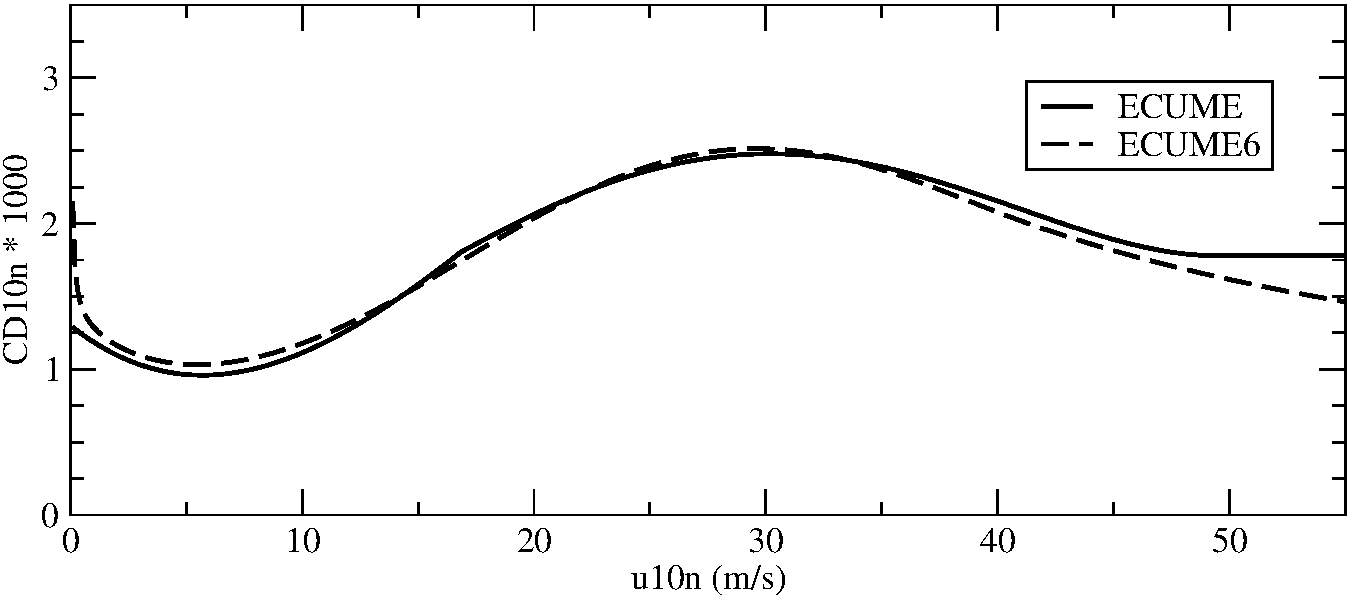
\includegraphics[width=19.4pc,clip=true]{\EPSDIR/new_cdn.pdf}
 \centering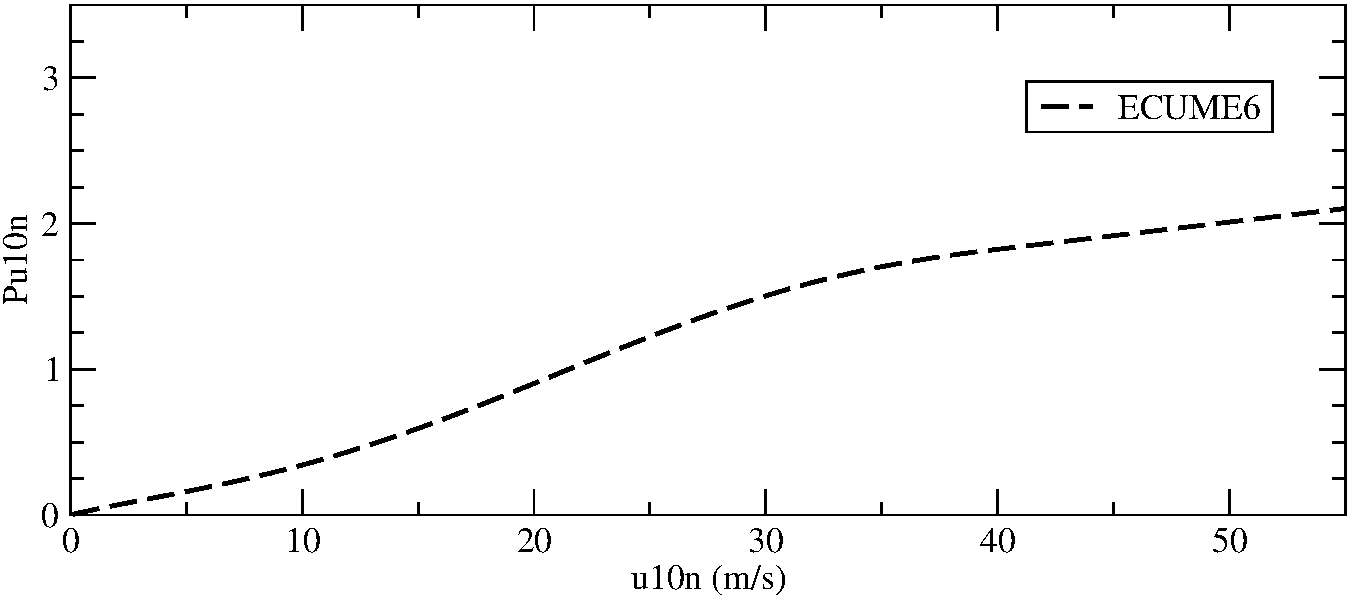
\includegraphics[width=19.4pc,clip=true]{\EPSDIR/parun.pdf}
 \centering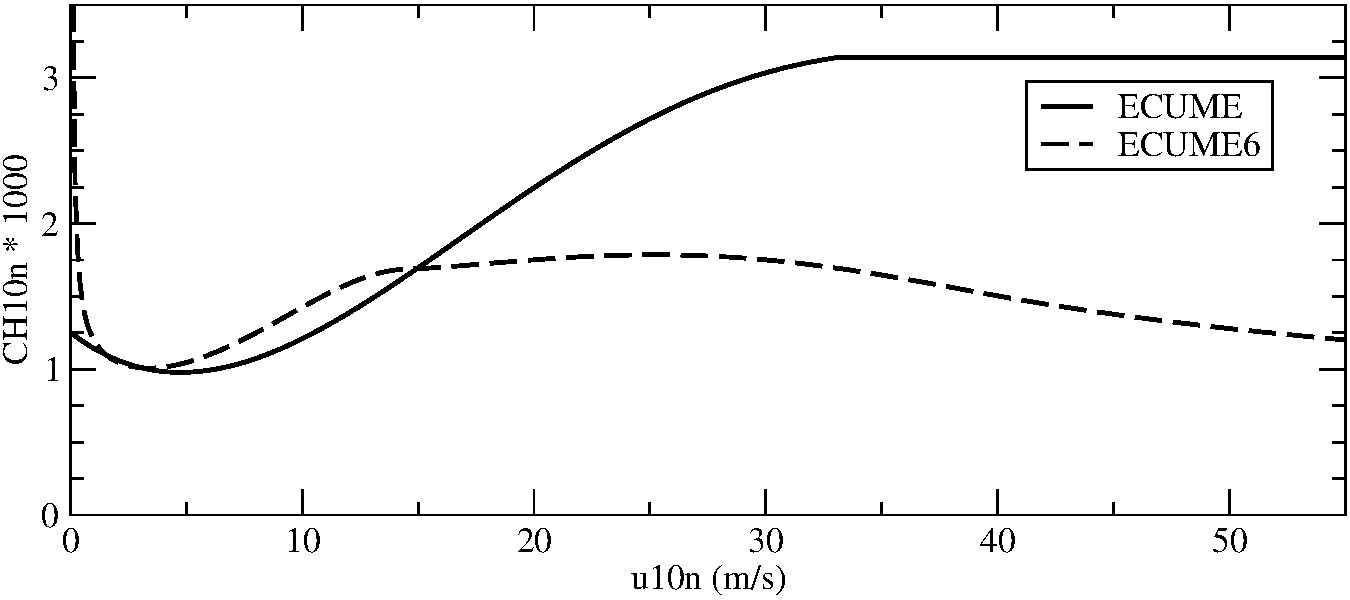
\includegraphics[width=19.4pc,clip=true]{\EPSDIR/new_chn.pdf}
 \centering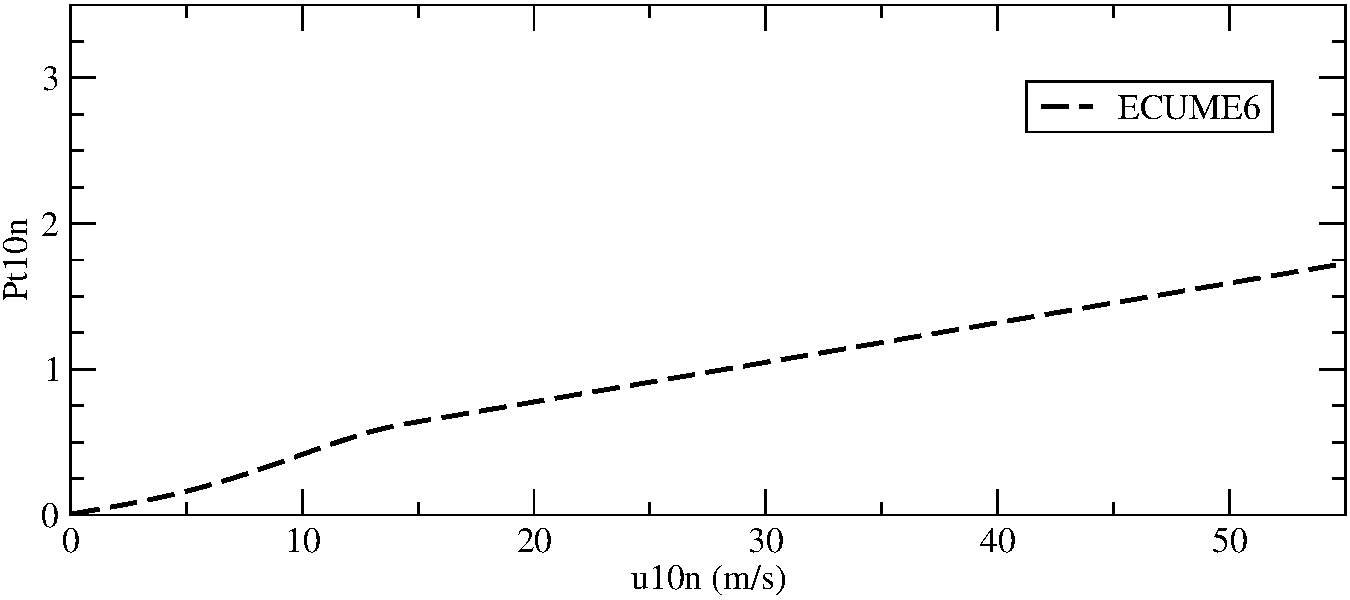
\includegraphics[width=19.4pc,clip=true]{\EPSDIR/partn.pdf}
 \centering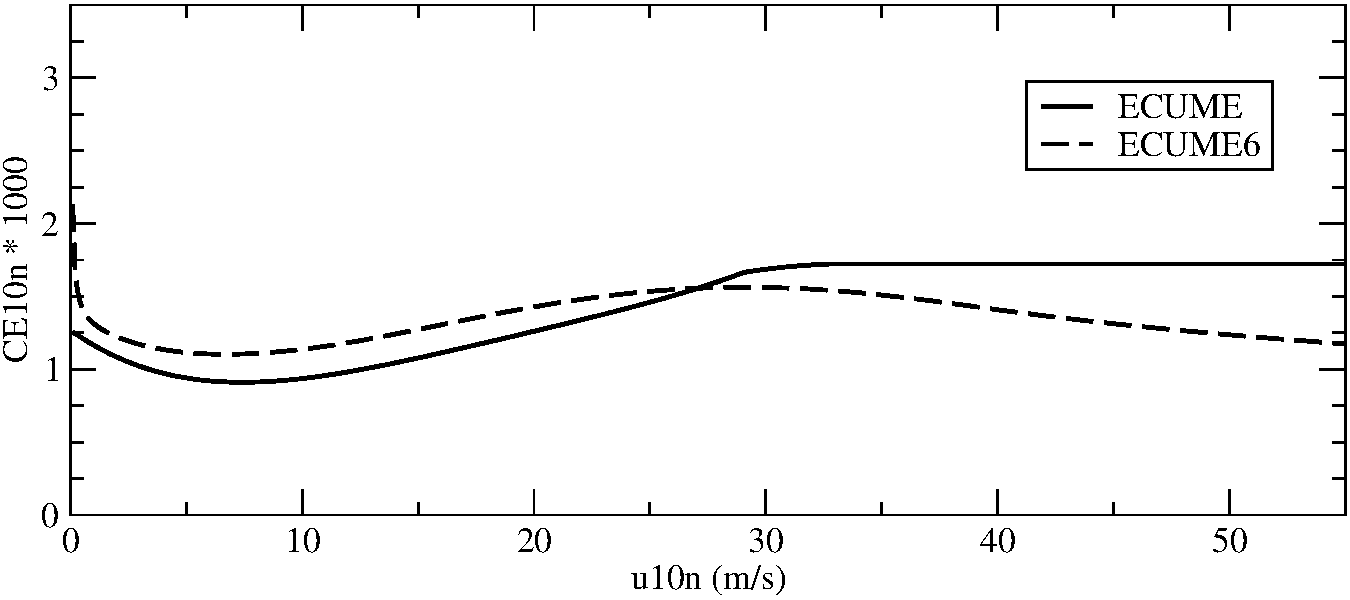
\includegraphics[width=19.4pc,clip=true]{\EPSDIR/new_cen.pdf}
 \centering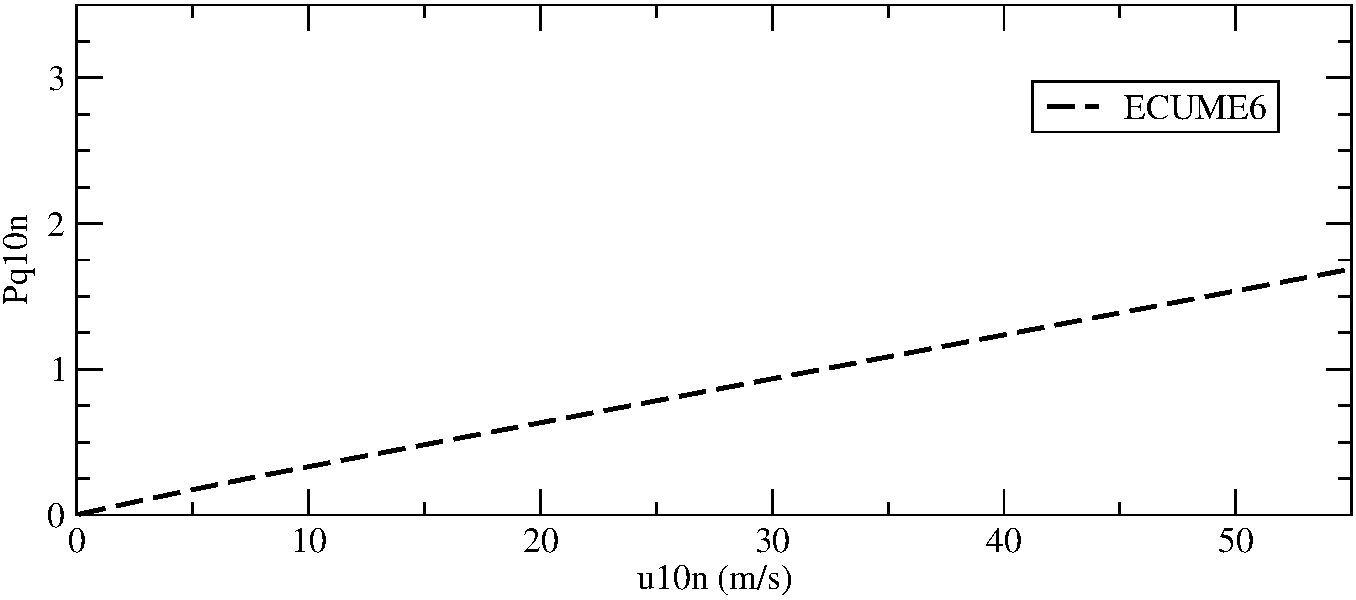
\includegraphics[width=19.4pc,clip=true]{\EPSDIR/parqn.pdf}
	\caption{Left: Neutral coefficients at 10 meters $C_{D_{10n}}$, $C_{H_{10n}}$ and $C_{E_{10n}}$ in the ECUME 
	(solid line) and derived from the ECUME6 (dashed line) formulations. 
	Right: Neutral parameters at 10 meters $\mathcal{P}_{u_{10n}}$, $\mathcal{P}_{{\theta}_{10n}}$ and $\mathcal{P}_{q_{10n}}$ 
	in the ECUME6 formulation.\label{ecume_coef}}
\end{figure}

The key difference between the two parameterizations is that the original one (\textit{ECUME}, see Belamari, 2005 %\citet{bel05}
for more details) provides formulations
of the neutral exchange coefficients at 10m (drag coefficient $C_{D_{10n}}$, heat coefficient $C_{H_{10n}}$ and 
evaporation coefficient $C_{E_{10n}}$) as functions of the neutral vertical wind gradient between the sea surface and 
10m-height $\Delta u_{10n}$ 
(Figure \ref{ecume_coef}, left part) while the new one (\textit{ECUME6}) provides formulations of derived parameters for the wind
$\mathcal{P}_{u_{10n}}$, potential temperature $\mathcal{P}_{{\theta}_{10n}}$ and specific humidity $\mathcal{P}_{q_{10n}}$
(Figure \ref{ecume_coef}, right part), defined as:
\begin{equation}
\left\{
\begin{array}{l}
	\mathcal{P}_{u_{10n}}=\left(\frac{C_{D_{10n}}}{\sqrt{C_{D_{10n}}}}\right)\times \Delta u_{10n} \\
	\mathcal{P}_{{\theta}_{10n}}=\left(\frac{C_{H_{10n}}}{\sqrt{C_{D_{10n}}}}\right)\times \Delta u_{10n} \\
	\mathcal{P}_{q_{10n}}=\left(\frac{C_{E_{10n}}}{\sqrt{C_{D_{10n}}}}\right)\times \Delta u_{10n} 
\end{array}
\right.
\end{equation}
The definition of these new parameters was motivated by the wide dispersion of the scatterplots providing the observed 
neutral exchange coefficients as a function of the neutral wind at 10 meters, in contrast to those of these new
parameters.\\

As in the two other iterative parameterizations, the ECUME and ECUME6 algorithms begin with a first \textbf{preliminary step} that insures the \textbf{initialization} 
of all the required variables, namely:
\begin{enumerate}
	\item the vertical gradients of the wind, potential temperature and specific humidity at the air-sea interface 
($\Delta u$, $\Delta \theta$ and $\Delta q$)
	\item the corresponding neutral vertical gradients:
$$
\left\{
\begin{array}{l}
	\Delta u_{10n}=\Delta u\\
	\Delta {\theta}_{10n}=\Delta \theta \times d_0\\
	\Delta q_{10n}=\Delta q
\end{array}
\right.
$$
with:
$$
\left\{
\begin{array}{ll}
	d_0=1.2+6.3~10^{-3}\mathit{MAX}(\Delta u-10~,~0) & \mathrm{in~ECUME}\\
	d_0=1.0 & \mathrm{in~ECUME6}
\end{array}
\right.
$$
\end{enumerate}
In ECUME6, an initial guess is also made for the characteristic length scales as initial values of 
$u_*$, ${\theta}_*$ and $q_*$ are required by the convergence criterion:
$$
\left\{
\begin{array}{l}
	u_*=0.04~\Delta u\\
	{\theta}_*=0.04~\Delta \theta\\
	q_*=0.04~\Delta q
\end{array}
\right.
$$

\vspace*{0.2 cm}

As a \textbf{second step}, the \textbf{iterative loop} then insures the computation of:
\begin{enumerate}
	\item the neutral exchange coefficients/parameters as functions of the neutral vertical wind gradient 
between the sea surface and 10m-height $\Delta u_{10n}$:
%%%%%%%%%%%%%%%%%%%%%%%%%
		\begin{center}
\begin{tabular}{|c|c|c|}
\hline
	 & ECUME & ECUME6 \\
\hline
	 & Neutral coefficient & Neutral parameter \\
	Momentum & $C_{D_{10n}}=f_u(\Delta u_{10n})$        & $\mathcal{P}_{u_{10n}}=g_u(\Delta u_{10n})$ \\
	Heat     & $C_{H_{10n}}=f_{\theta}(\Delta u_{10n})$ & $\mathcal{P}_{{\theta}_{10n}}=g_{\theta}(\Delta u_{10n})$ \\
	Moisture & $C_{E_{10n}}=f_q(\Delta u_{10n})$        & $\mathcal{P}_{q_{10n}}=g_q(\Delta u_{10n})$ \\
\hline
\end{tabular}
		\end{center}
%%%%%%%%%%%%%%%%%%%%%%%%%

	\item the characteristic length scales $u_*$, ${\theta}_*$ and $q_*$ derived from the previous coefficients/parameters:
%%%%%%%%%%%%%%%%%%%%%%%%%
		\begin{center}
\begin{tabular}{|c|c|c|}
\hline
	 & ECUME & ECUME6 \\
\hline
	 & \multicolumn{2}{c|}{Scaling parameters}\\
	Momentum & $u_*=\sqrt{C_{D_{10n}}}.\Delta u_{10n}$  & $u_*=\mathcal{P}_{u_{10n}}$ \\
	Heat     & ${\theta}_*=\left(\frac{C_{H_{10n}}}{\sqrt{C_{D_{10n}}}}\right).\Delta {\theta}_{10n}$  
			& ${\theta}_*=\mathcal{P}_{{\theta}_{10n}}\left(\frac{\Delta {\theta}_{10n}}{\Delta u_{10n}}\right)$ \\
	Moisture     & $q_*=\left(\frac{C_{E_{10n}}}{\sqrt{C_{D_{10n}}}}\right).\Delta q_{10n}$  
			& $q_*=\mathcal{P}_{q_{10n}}\left(\frac{\Delta q_{10n}}{\Delta u_{10n}}\right)$ \\
\hline
\end{tabular}
		\end{center}
%%%%%%%%%%%%%%%%%%%%%%%%%
	\item the stability parameter $\zeta$=$z/L$ constrained to be in the range $[$-200.0;0.25$]$,
using for the Monin-Obukhov length $L$ the same approximate formulation as in COARE3.0
(equation \ref{LMO_approx})
	\item the stability functions $\psi_{m}$ and $\psi_{h}$ as $\psi_{q}$ is supposed to be equal to $\psi_{h}$ (section \ref{iterative_param}.4)
	\item and last, the neutral vertical gradients:
$$
\left\{
\begin{array}{l}
\vspace*{0.2 cm}
	\Delta u_{10n}=\Delta u - \frac{u_*}{\kappa}\left[\ln\left(\frac{z}{10}\right)-{\psi}_m(\zeta)\right]\\
\vspace*{0.2 cm}
	\Delta {\theta}_{10n}=\Delta {\theta} - \frac{{\theta}_*}{\kappa}\left[\ln\left(\frac{z}{10}\right)-{\psi}_h(\zeta)\right]\\
	\Delta q_{10n}=\Delta q - \frac{q_*}{\kappa}\left[\ln\left(\frac{z}{10}\right)-{\psi}_q(\zeta)\right]
\end{array}
\right.
$$
\end{enumerate}

\textbf{At the end of the iterative loop}, the final values of the characteristic length scales are then used to derive:
\begin{itemize}

	\item the exchange coefficients $C_D$, $C_H$ and $C_E$ (from equations \ref{eq_COEF}),

	\item the air-sea turbulent fluxes ${\tau}_{\mathit{sea}}$, $H_{\mathit{sea}}$ and ${\mathit{LE}}_{\mathit{sea}}$ 
	(from equations \ref{eq_bulk} in ECUME and \ref{eq_charlength} in ECUME6),

	\item and last, the roughness lengths:
\begin{itemize}
	\item in ECUME, the dynamical roughness length $z_0$ is computed in a single way using the \textit{subgrid} formulation 
(equation \ref{z0_arpege}) with $\beta$=10$^{-5}$

	\item in ECUME6, the dynamical roughness length $z_0$ may be computed in three different ways depending on the 
choice of a dedicated parameter (\textit{KZ0}):
\begin{itemize}
	\item using the \textit{subgrid} formulation with $\beta$=10$^{-5}$ in equation \ref{z0_arpege} if \textit{KZ0}=0
	\item using the relationship of Smith (1988) with $\beta$=0.11 in equation \ref{z0_smith} if \textit{KZ0}=1
	\item from the characteristic length scale $u_*$, using a formulation derived from equation \ref{allstars} if \textit{KZ0}=2:
\begin{equation}
	z_0=z \left(\exp \left[\kappa\frac{\Delta u}{u_*}+{\psi}_m(\zeta)\right]\right)^{-1}
\label{z0_direct}
\end{equation}
\end{itemize}
\end{itemize}
Note that if the dynamical roughness length $z_0$ is computed using the \textit{subgrid} formulation or the relationship of Smith (1988),
the Charnock parameter $\alpha$ may be either constant  
if \textit{CCHARNOCK=\textquotesingle{}OLD\textquotesingle{}} (then $\alpha$=0.021)
or wind dependent as in COARE3.0 (equation \ref{charnockwithwind}) 
if \textit{CCHARNOCK=\textquotesingle{}NEW\textquotesingle{}}.
\end{itemize}

The ECUME and ECUME6 parameterizations include other specific points:

\begin{enumerate}

	\item No waves effects are taken into account in these parameterizations. 

	\item A stochastic perturbation may be applied to the air-sea turbulent fluxes (logical \textit{OPERTFLUX}) in both
parameterizations.

	\item In ECUME, the number of iterations is prescribed (fixed to 10), while in ECUME6 a convergence criterion is used:
the iterative loop is stopped when the difference between the scale parameters of two successive iterations is 
inferior to a prescribed threshold ($10^{-6}$ ms$^{-1}$ for $u_{*}$, $10^{-6}$ K for $\theta_{*}$ and $10^{-9}$ kg/kg for $q_{*}$).
Note that an important effort was done for the ECUME6 algorithm in order to ensure the convergence in maximum 10 iterations 
whatever the meteo-oceanic conditions (Belamari, 2005). %\citep{bel05}

	\item In ECUME, a correction may be applied to the neutral coefficient for humidity (default is \textit{XICHCE}=0):

		$C_{E_{10n}}=C_{E_{10n}}(1-\mathit{XICHCE})+C_{H_{10n}}(\mathit{XICHCE})~~~~~\mathrm{with}~~~~~0.0\leq\mathit{XICHCE}\leq1.0$


\end{enumerate}


\subsubsection{\ref{iterative_param}.4 $~$ Stability functions used in the iterative parameterizations}

The stability functions $\psi_{m}$ and $\psi_{h}$ used in the four iterative parameterizations 
to correct the wind, potential temperature and specific humidity logarithmic profiles in the boundary layer 
according to the atmospheric stratification are all modified Businger's %\nocite{bus71}
functions as detailed hereafter. ECUME* stands for both ECUME and ECUME6, and ${\psi}_*$ represents either
$\psi_{m}$ or $\psi_{h}$ depending on the considered parameter.

You may note that in unstable conditions the stability functions result from two contributions: a \textit{Kansas} part
to represent the classical unstability, and a \textit{Convective} part to take into account the free convection,
with a weight $f$ depending on the Monin-Obukhov stability parameter $\zeta$.
In the MR98 parameterization, a different formulation is used for the weight $f$ but we do not
mention it here as the resulting formulation of the stability functions including the two contributions is 
rigorously equivalent.

%%%%%%%%%%%%%%%%%%%%%%%%%
\begin{table}[!h]
\centering
\begin{tabular}{|c|lc|c|}
\hline
	& & Wind & Potential temperature \\
\hline
	& & & \\
	Stable         & \textbf{MR98}     & \multicolumn{2}{c|}{$\psi_{*}(\zeta)=-4.7~\zeta$}\\
	($\zeta\geq0$) & \textbf{ECUME*}   & \multicolumn{2}{c|}{$\psi_{*}(\zeta)=-7.0~\zeta$}\\
	               & \textbf{COARE3.0} & \multicolumn{2}{c|}{$\psi_{*}(\zeta)=-\left[1+\zeta+\frac{2}{3}\left(\frac{\zeta-14.28}{\exp(\Gamma)}\right)+8.525\right]~~\mathrm{with}~~\Gamma=\mathit{MIN}(50,~0.35\zeta)$}\\
	& & & \\
\hline
	& & & \\
	Unstable    & & \multicolumn{2}{c|}{$\psi_{*}(\zeta)=(1-f)\psi_{*K}+f\psi_{*C}$}\\
	($\zeta<0$) & & \multicolumn{2}{c|}{with $~~f=\frac{\zeta^{2}}{1+\zeta^{2}}$}\\
	& & & \\
	Kansas      & & $\psi_{mK}=2.\ln\left(\frac{1+x}{2}\right)+\ln\left(\frac{1+x^{2}}{2}\right)$ & $\psi_{hK}=2.\ln(\frac{1+x^2}{2})$\\
	            & & $-2.\arctan(x)+\frac{\pi}{2}$ & \\
	            & & \multicolumn{2}{c|}{with:} \\
	            & \textbf{MR98}     & \multicolumn{2}{c|}{$x=(1-16~\zeta)^{\frac{1}{4}}$}\\
		    & \textbf{ECUME*}   & \multicolumn{2}{c|}{$x=(1-16~\zeta)^{\frac{1}{4}}$}\\
		    & \textbf{COARE3.0} & \multicolumn{2}{c|}{$x=(1-15~\zeta)^{\frac{1}{4}}$}\\
	            & & & \\
	Convective  & & \multicolumn{2}{c|}{$\psi_{*C}=\frac{3}{2}\ \ln\left(\frac{1+y+y^2}{3}\right)-\sqrt{3}.\arctan\left(\frac{1+2y}{\sqrt{3}}\right)+\frac{\pi}{\sqrt{3}}$}\\
	            & & \multicolumn{2}{c|}{with:} \\
	            & \textbf{MR98}     & \multicolumn{2}{c|}{$y=(1-12.87~\zeta)^{\frac{1}{3}}$}\\
		    & \textbf{ECUME*}   & \multicolumn{2}{c|}{$y=(1-12.87~\zeta)^{\frac{1}{3}}$}\\
		    & \textbf{COARE3.0} & $y=(1-10.15~\zeta)^{\frac{1}{3}}$ & $y=(1-34.15~\zeta)^{\frac{1}{3}}$ \\
	   & & & \\
\hline
\end{tabular}
\caption{Stability functions used in the iterative parameterizations.
\label{stability_functions}}
\end{table}
%%%%%%%%%%%%%%%%%%%%%%%%%

\vspace*{0.2 cm}


\subsubsection{\ref{iterative_param}.5 $~$ Additional refinements included in the iterative parameterizations}

Each of the four iterative parameterizations may include some refinements as detailed in Table \ref{refinements}.
\begin{enumerate}

	\item \textbf{Salinity correction:} 
A reduction of 2\% may be applied to the saturated vapor pressure $P_{\mathit{sat}}$ used in the computation 
of the specific humidity at the sea surface $q_s$ in order to take into account the decreasing of $P_{\mathit{sat}}$
due to seawater salinity (Kraus, 1972)\nocite{kraus1972}:  
\begin{equation}
	q_{s}=q_{s}(P_{\mathit{sat}})~~~~~\mathrm{with}~~~~~P_{\mathit{sat}}=0.98\times P_{\mathit{sat}}(T_{s})
\end{equation}

	\item \textbf{Explicit dependency to sea surface salinity:}
In ECUME6, if the sea surface salinity (SSS) field is available in the SURFEX surface scheme, an explicit dependency to the SSS
may be used in the computation of both the saturated vapor pressure $P_{\mathit{sat}}$ from which the specific humidity at 
the sea surface $q_s$ is derived (Sharqawy \textit{et al.}, 2010), %\citet{Sharqawy2010}
and the latent heat of seawater vaporization ${\mathcal{L}}_{v}$:
$$
\left\{
\begin{array}{l}
	q_{s}=q_{s}(P_{\mathit{sat}})~~~~~\mathrm{with}~~~~~P_{\mathit{sat}}=P_{\mathit{sat}}(T_{s},SSS)\\
	{\mathcal{L}}_{v}={\mathcal{L}}_{v}(\mathit{SSS})
\end{array}
\right.
$$

	\item \textbf{Wind subgrid correction:}
The relative wind - and therefore the wind gradient - may be increased by a subgrid correction ($w_g$) introduced in order to 
take into account the gustiness impact:
\begin{equation}
	\Delta u=\sqrt{U^2+{w_g}^2}~~~~~~~~~~\mathrm{with}~~~~~~~~~~w_g={\beta}_{\mathit{gust}}({B_F}.z_{\mathit{BL}})^{\frac{1}{3}}
\end{equation}
$z_{\mathit{BL}}$ is the atmospheric boundary layer depth (in meters), ${\beta}_{\mathit{gust}}$ is a constant coefficient,
and ${B_F}$ is the surface buoyancy flux:
		$${B_F}=-g.u_*.\mathcal{F}$$
If $B_F \leq$0, the wind correction $w_g$ is set to a minimal value $w_{g_{\mathit{min}}}$.

	\item \textbf{Wind stress correction} and \textbf{Heat flux correction} due to rainfall:
As rainfall tends to increase the surface drag and to cool the ocean, two additional contributions 
$\tau_{r}$ (Fairall \textit{et al.}, 1996b) %\citep{fbr96}
and $H_{r}$ (Gosnell \textit{et al.}, 1995) %\citep{gfw95}
may be computed in order to correct the surface wind stress and sensible heat flux, respectively:
\begin{equation}
\left\{
\begin{array}{l}
	{\tau}_r=-\gamma~\mathcal{R} \times U\\
	H_r={\mathcal{R}}~{c_{p_{\mathit{lw}}}} {\alpha}_c (T_s-T_a)\left(1+\frac{1}{B}\right)
\end{array}
\right.
\end{equation}
$\mathcal{R}$ denotes the precipitation rate (in kg.s$^{-1}$.m$^{-2}$).
$c_{p_{\mathit{lw}}}$ is the rain specific heat including a dependency to the rain temperature (supposed to be equal to that of the air).
${\alpha}_c$ is a dimensionless parameter called the wet-bulb factor:
\begin{equation}
	{\alpha}_c=\left[1+ \frac{L_r~d_v}{c_{p_d}~d_h} \left(\frac{dq_{\mathit{sat}}}{dT}\right) \right]^{-1}
\end{equation}
where $L_r$ is the latent heat of rain vaporization (in J.kg$^{-1}$), 
$c_{p_d}$ is the specific heat of dry air (in J.K$^{-1}$.kg$^{-1}$),
$d_v$ and $d_h$ are the diffusivities for water vapor (Pruppacher and Klett, 1978) and heat, respectively.
The slope of the saturated specific humidity at atmospheric level $q_{\mathit{sat}}({\theta}_a)$ as a function of the temperature 
is derived from the Clausius-Clapeyron relation:
		$$\frac{dq_{\mathit{sat}}}{dT}=\lambda \left[ \frac{L_r~q_{\mathit{sat}}({\theta}_a)}{R_v~{T_a}^{2}}\right]$$
$B$ is the Bowen ratio:
	$$B= \mu \left(\frac{c_{p_d}}{L_r}\right) \left(\frac{T_s-T_a}{q_s-q_a}\right)$$

	\item \textbf{Webb correction:}
%\nocite{wbb80}
This small correction may be applied to the latent heat flux in order to take into account the air density variations when the humidity 
varies under the evaporation action:
$$LE_{\mathit{Webb}}=\rho_{a}~{\mathcal{L}}_{v}~\overline{w}~q_a$$
where ${\mathcal{L}}_{v}$ is the latent heat of seawater vaporization at sea surface, and $\overline{w}$ is the mean value of the vertical 
speed perturbations: 
$$ \overline{w} = 1.61~\overline{w'q'}+(1+1.61~q_a)\frac{\overline{w'{\theta}'}}{T_a} = -\left[1.61~u_* q_*+(1+1.61~q_a)\frac{u_* {\theta}_*}{T_a}\right] $$

\end{enumerate}

%%%%%%%%%%%%%%%%%%%%%%%%%
\begin{table}[!h]
\centering
\begin{tabular}{|l|c|c|c|c|}
\hline
	                       	& MR98                                              & COARE3.0 & ECUME & ECUME6 \\
\hline
	Salinity correction    	& Yes                                               & Yes      & Yes   & Yes    \\
\hline
	Explicit dependency  	& No                                                & No       & No    & Yes [1] \\
	to sea surface salinity & & & & \\
\hline
				& Yes with:                                         & Yes [2] with: & Yes [2] with: & No \\
				& $w_{g_{\mathit{min}}}$=0.0 ms$^{-1}$              & $w_{g_{\mathit{min}}}$=0.2 ms$^{-1}$ & $w_{g_{\mathit{min}}}$=0.0 ms$^{-1}$ & \\
	Wind subgrid		& ${\beta}_{\mathit{gust}}$=0.6                     & ${\beta}_{\mathit{gust}}$=1.2 & ${\beta}_{\mathit{gust}}$=1.2 & \\
	correction              & $z_{\mathit{BL}}$=650 m                           & $z_{\mathit{BL}}$=600 m & $z_{\mathit{BL}}$=600 m & \\
		       		& $\mathcal{F}=\frac{{{\theta}_v}_{*}}{{\theta}_v}$ 
				& $\mathcal{F}=\frac{{\theta}_{*}+0.61(T_a q_*)}{T_a}$ 
				& $\mathcal{F}=\frac{{{\theta}_v}_{*}-0.61({\theta}_a-T_a)q_*}{T_a}$ & \\
	 			& & & & \\
\hline
	Wind stress correction  & No & Yes [3] with  & Yes [3] with & Yes [3] with  \\
	due to rainfall         &    & $\gamma$=0.85 & $\gamma$=1.0 & $\gamma$=0.85 \\
\hline
	    			& No & Yes with:   & Yes with:                 & Yes with:                 \\
	Heat flux correction    &    & $\lambda$=1 & $\lambda=\frac{R_v}{R_d}$ & $\lambda$=1 \\
	due to rainfall		&    & $\mu$=1     & $\mu=\frac{d_h}{d_v}$     & $\mu=\frac{d_h}{d_v}$ \\
	 			& & & & \\
\hline
\multicolumn{5}{|l|}{[1] If the sea surface salinity field is available in the SURFEX surface scheme.} \\
\multicolumn{5}{|l|}{$~~~~~$ Else, only the standard ``Salinity correction'' is applied.} \\
\hline
\multicolumn{5}{|l|}{[2] Logical \textit{LPWG} in the \textit{NAM\_SEAFLUXn} namelist.} \\
\hline
\multicolumn{5}{|l|}{[3] Logical \textit{LPRECIP} in the \textit{NAM\_SEAFLUXn} namelist.} \\
\hline
\end{tabular}
	\caption{Additional refinements available (or not) in the iterative parameterizations.
\label{refinements}}
\end{table}
%%%%%%%%%%%%%%%%%%%%%%%%%

Note that:
\begin{enumerate}
	\item In the various formulations of the surface buoyancy flux $B_F$, ${\theta}_v$ is the air virtual potential temperature
(equation \ref{eq_thetav}), ${{\theta}_v}_{*}$ is the associated characteristic length scale given by equation \ref{eq_thetavstar}, 
${\theta}_a$ and $T_a$ are the air potential temperature and air temperature, respectively. 
This leads to different formulations in COARE3.0 and ECUME when compared to the (exact) one used in MR98.
	\item In the heat flux correction due to rainfall, $\lambda$ and $\mu$ should be equal to 1 to be fully consistent with 
Gosnell \textit{et al.} (1995). %\citet{gosnell1995}
\end{enumerate}

%%%%%%%%%%%%%%%%%%%%%%%%%%%%%%%%%%%%%%%%%%%%%%%%%%%%%%%%%%%%%%%%%%%%%%%%%%%%%%%%%%%%%%%%%%%%%%%%%%%%%%%%%%%%%%%%%%%%%%%%

\newpage
\section{Coupling with a 1D TKE oceanic model}
\subsection{Coupling objectifs and principles}
The main objective of the coupling is to improve the fine scale air-sea exchanges modelling in the SURFEX surface scheme. To better represent the fine scale air-sea interactions, it is necessary to take into account the oceanic dynamics and the thermal content evolution (Lebeaupin \etal (2007, 2009)) %\citep{leb08a,leb08b}
. \\
\begin{figure}[!b]
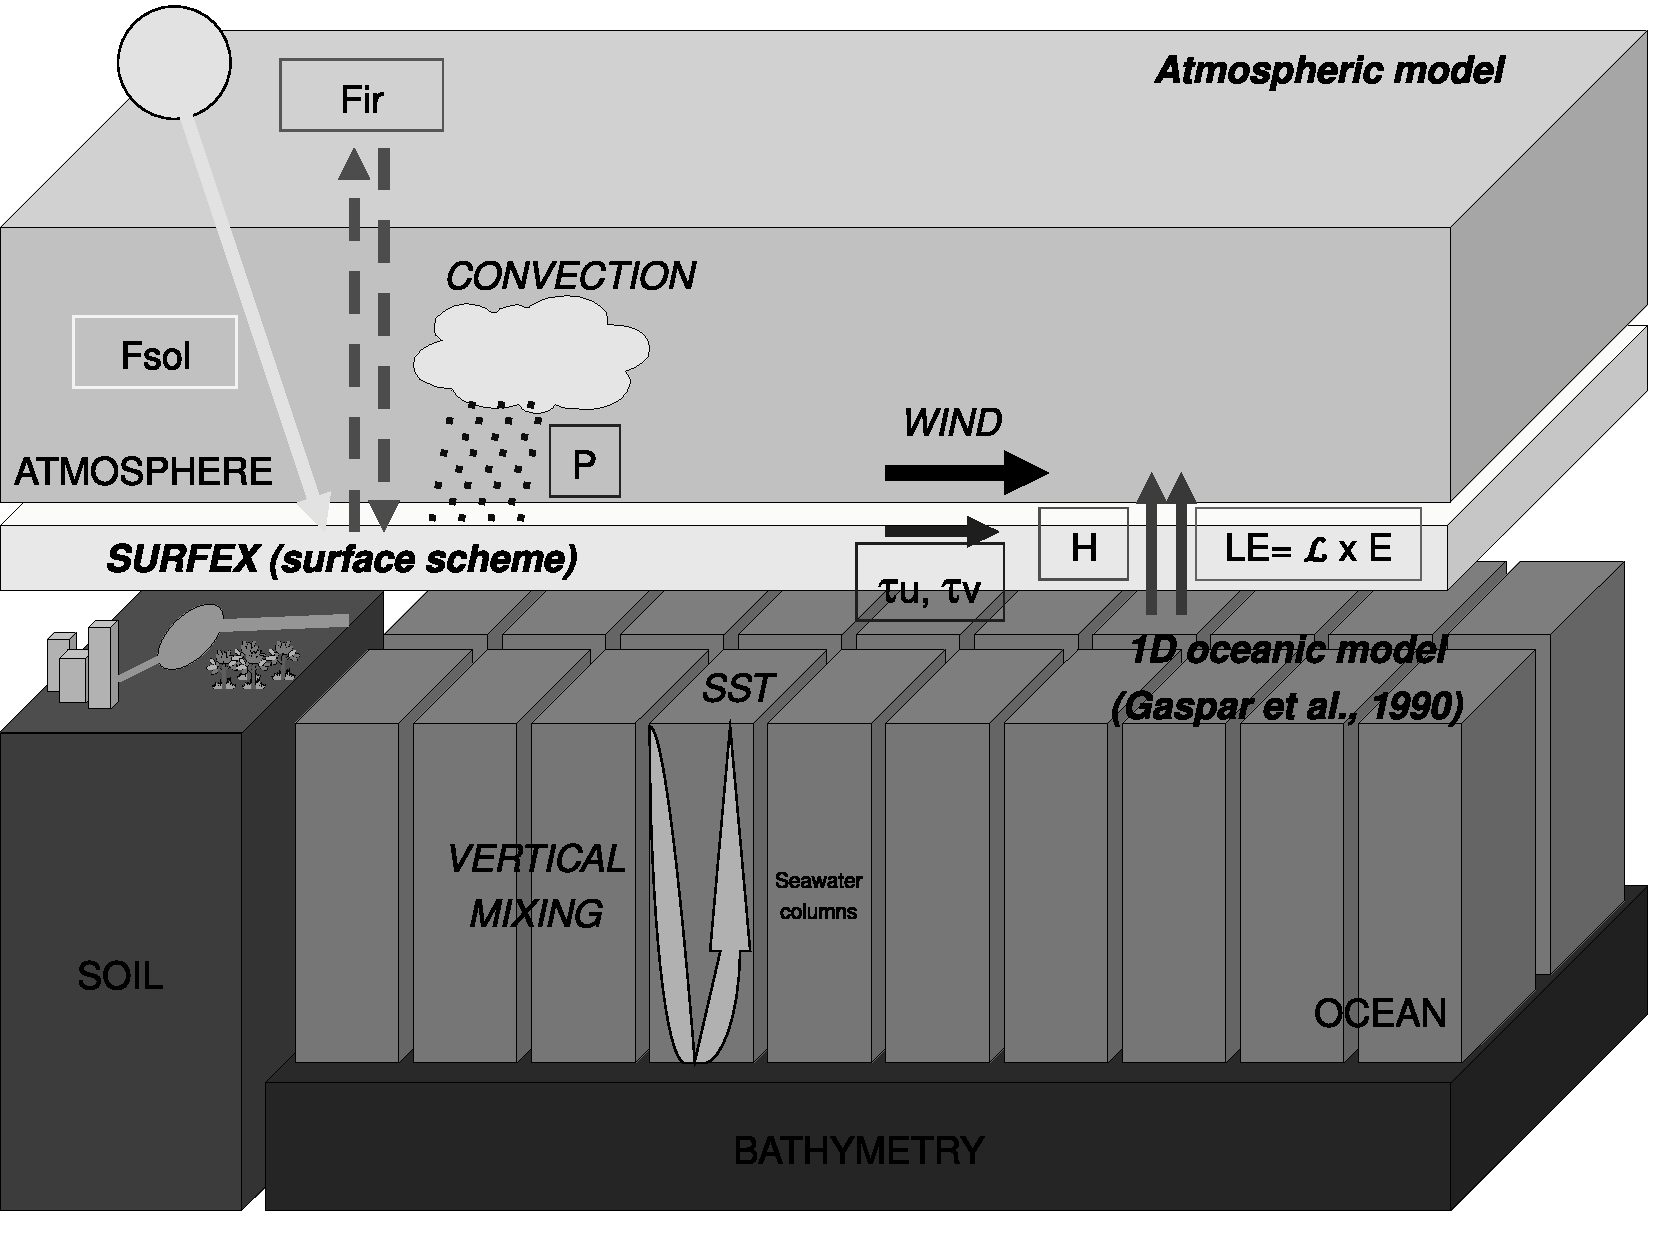
\includegraphics[width=37pc]{\EPSDIR/coupling_scheme+processes.NB.pdf}
\vspace{-0.75cm}
\caption{The high-resolution ocean-atmosphere coupled system between (MESO-NH) SURFEX and the 1D oceanic model. \label{scheme_coupled_syst}}
\end{figure}
 
The coupled system's principle consists in modelling a seawater column under each grid point containing a fraction of sea and limited by the bottom (Figure \ref{scheme_coupled_syst}). The ocean model used is the uni-dimensional model described by Gaspar \etal (1990) \nocite{Gaspar1990}
 [see section \ref{sct_mod1d}] which allows to represent the oceanic vertical mixing according to a parameterization of turbulence from Bougeault and Lacarr\`ere (1989)\nocite{BL89}
 adapted to ocean. By the turbulent vertical mixing modelling, the 1D ocean model allows to represent the heat, water and momentum exchanges from the superficial oceanic layers in direct interaction with the atmosphere and subjected to radiative effects, to the deepest layers. The turbulent vertical mixing is based on a parameterization of the second-order turbulent moments expressed as a function of the turbulent kinetic energy (Gaspar \etal, 1990). In this formulation, the vertical mixing coefficients are based on the calculation of two turbulent length scales representing upward and downward conversions of turbulent kinetic energy (TKE) into potential energy (Gaspar \etal, 1990). By allowing a response to high frequencies in the surface forcing, the scheme improved the representation of the vertical mixed layer structure, sea surface temperature and upper-layer current (Blanke and Delecluse, 1993 \nocite{Blanke1993}). However, this parameterization fails to properly simulate the mixing in strongly stable layers in the upper thermocline (Large\etal, 1994 \nocite{Large1994}; Kantha and Clayson, 1994 \nocite{Kantha1994}). Consequently, a parameterization of the diapycnal mixing (Large \etal, 1994) was introduced into Gaspar's turbulence parameterization model in order to take into account the effects of the vertical mixing occurring in the thermocline (Josse, 1999 \nocite{Josse1999}). This non local source of mixing, mainly due to internal wave breaking and current shear between the mixed layer and upper thermocline, impacts the temperature, salinity, momentum and turbulent kinetic energy inside the mixed layer particularly during restratification periods. This parameterization was widely used, for instance to study successfully the diurnal cycle in the Equatorial Atlantic (Wade \etal, 2011 \nocite{Wade2011}), the Equatorial Atlantic cold tongue (Giordani \etal, 2011 \nocite{Giordani2011}), the production of modal waters in the North-East Atlantic (Giordani \etal, 2005b \nocite{Giordani2005b}) or to derive surface heat flux corrections (Caniaux \etal, 2005b \nocite{Caniaux2005b}). Note that horizontal and vertical advections can be easily prescribed in the 1D-mixing model to perform realistic simulations in heterogeneous situations.

\subsection{Description of the 1D oceanic model in TKE equation \label{sct_mod1d}}
The 1D model includes a prognostic equation for the turbulent kinetic energy (e) with a 1.5 order closure. The other prognostic variables are the temperature (T), the salinity (S), and the current [$\vec{u}=(u,v)$]. 

\subsubsection{Prognostic equations for T, S, u and v}
Each of the prognostic variables ($\alpha$) is decomposed in a mean value ($\overline{\alpha}$) and a perturbation around this mean value ($\alpha '$), so $\alpha=\overline{\alpha}+\alpha '$. 
For each seawater column, T, S, u and v evolve under the turbulent vertical mixing effect. This mixing depends of air-sea interface fluxes. 

The conservative equations are:
\begin{equation}
\left\{
\begin{array}{l}
\frac{\partial T}{\partial t}=\frac{F_{sol}}{\rho_{0}c_{p}}\frac{\partial I(z)}{\partial z}-\frac{\partial \overline{T'w'}}{\partial z}\\
\\
\frac{\partial S}{\partial t}=-\frac{\partial \overline{S'w'}}{\partial z}\\
\\
\frac{\partial \vec{u} 
}{\partial t}=-f\vec{k}\times \vec{u}-\frac{\partial \overline{\vec{u}'w'}}{\partial z}
\end{array}
\right.
\end{equation}

\noindent where $w$ is the vertical velocity, $\rho_{0}$ is a reference density, $c_{p}$ is the specific heat, $f$ is the Coriolis parameter. $\vec{k}$ is the unit vertical along the vertical, $F_{sol}$ is the solar radiation received by the surface, and $I(z)$ is the solar radiation fraction reaching the depth z ($I(z)$ function decreases exponentially with depth). 

The conditions at the top of the model (z=0) are:
\begin{equation}
\left\{
\begin{array}{l}
-\overline{T'w'}(0)=\frac{F_{nsol}}{\rho_{0}c_{p}}=\frac{H+LE+F_{ir}}{\rho_{0}c_{p}}\\
\\
-\overline{S'w'}(0)=\frac{E-P}{\rho_{0}c_{p}}\\
\\
-\overline{\vec{u}'w'}(0)=\frac{\vec{\tau}}{\rho_{0}c_{p}}\\
\end{array}
\right.
\label{eq_mod1D_interface}\end{equation}

\textbf{Fluxes are positive here downwards. }\\

Finally, the forcing variables to give to the oceanic model are:
\begin{itemize}
\item the solar radiation $F_{sol}$
\item the infra-red radiation $F_{ir}$
\item the evaporation rate $E$ proportional to the latent heat flux $E=\frac{LE}{\mathcal{L}}$
\item the sensible heat flux $H$
\item the zonal and meridional stress components $\vec{\tau}=(\tau_{u},\tau_{v})$
\item the precipitation rate $P$
\end{itemize}
$F_{nsol}$ is defined as the sum of the sensible H, the latent heat flux LE and the infra-red radiation $F_{ir}$ and is named non-solar flux. 


The closure relationships are given by: 
\begin{equation}
\left\{
\begin{array}{l}
-\overline{T'w'}=K_{h}\frac{\partial \overline{T}}{\partial z}\\
\\
-\overline{S'w'}=K_{s}\frac{\partial \overline{S}}{\partial z}\\
\\
-\overline{\vec{u}'w'}=K_{m}\frac{\partial \overline{\vec{u}}}{\partial z}
\end{array}
\right.
\end{equation}

The $K_{*}$ are diffusivity coefficients linked to the turbulent kinetic energy by: 
\begin{equation}
K=c_{k}l_{k}\overline{e}^{\frac{1}{2}}=K_{h}=K_{s}=\frac{K_{m}}{Prt}\simeq K_{m}
\end{equation}

\noindent where $c_{k}$ is a constant to determine; $l_{k}$ is a mixing length and $Prt$ is the Prandlt's number. 

\subsubsection{Prognostic equation for turbulent kinetic energy}
The equation for TKE $e=\frac{1}{2}(u'^{2}+v'^{2}+w'^{2})$ is given by:
\begin{equation}
\frac{\partial \overline{e}}{\partial t}=-\frac{\partial}{\partial z}\left(\overline{e'w'}+\frac{\overline{p'w'}}{\rho_{0}}\right)-\overline{\vec{u'}w'}\times \frac{\partial \overline{\vec{u}}}{\partial z}+\overline{b'w'}-\epsilon
\end{equation}
\noindent where $p$ is pressure; $\epsilon=c_{\epsilon}l_{\epsilon}\overline{e}^{\frac{3}{2}}$ is dissipation; $b=g\frac{\rho-\rho_{0}}{\rho_{0}}$ is the buoyancy. The seawater density is diagnosed from temperature and salinity:
$$\rho=\rho_{0}+(T-T_{ref})\times[-0.19494-0.49038(T-T_{ref})]+0.77475(S-S_{ref})$$
where $T_{ref}=13.5$ °C, $S_{ref}=32.6$ psu and $\rho_{0}=1024.458$ kg/m$^{3}$. 

The vertical TKE flux is parameterized:
\begin{equation}
-\left(\overline{e'w'}+\frac{\overline{p'w'}}{\rho_{0}}\right)=K_{e}\frac{\partial \overline{e}}{\partial z}
\end{equation}
with
\begin{equation}
K_e=c_{\epsilon}l_{\epsilon}\overline{e}^{\frac{1}{2}}
\end{equation}

The Bougeault and Lacarr\`ere %\citet{bou89}
 mixing length are:
\begin{equation}
l_{\epsilon}=(l_{u}l_{d})^{\frac{1}{2}}
\end{equation}
\begin{equation}
l_{k}=min(l_{u},l_{d})~ pour~k=h,s~and~m
\end{equation}

$l_{u}$ and $l_{d}$ (for ``up'' and ``down'') are estimated as the upwards and downwards distances for which the kinetic energy is transformed in potential energy:
\begin{equation}
\overline{e}(z)=\frac{g}{\rho_{0}}\int_{z}^{z+l_{u}}\lbrack\overline{\rho}(z)-\rho(z')\rbrack dz'
\end{equation} 
\begin{equation}
\overline{e}(z)=\frac{g}{\rho_{0}}\int_{z}^{z-l_{d}}\lbrack\overline{\rho}(z)-\rho(z')\rbrack dz'
\end{equation} 

\subsubsection{Discretization}
The temporal integration scheme is a semi-implicit scheme for T and S. For the horizontal current $\vec{u}=(u,v)$, the integration scheme is implicit/semi-implicit. 

The discretization is here described in detail for the temperature. The same could be done for the salinity, the TKE and the current in complex notation ($\vec{u}\rightarrow u+iv$, $i^{2}=-1$). 

The equation
$$
\frac{\partial T}{\partial t}=\frac{F_{sol}}{\rho_{0}c_{p}}\frac{\partial I(z)}{\partial z}-\frac{\partial}{\partial z}\left(-K\frac{\partial \overline{T}}{\partial z}\right)$$
is decomposed as:
\begin{equation}
\frac{T^{t+1}_{k}-T^{t}_{k}}{\Delta t}=\frac{F_{sol}}{\rho_{0}c_{p}}\frac{\partial I(z)}{\partial z}+\frac{1}{\Delta z_{2}(k)}\lbrack K(k+1)\frac{T^{t+1}_{k+1}-T^{t+1}_{k}}{\Delta z_{1}(k)}-K(k)\frac{T^{t+1}_{k}-T^{t+1}_{k-1}}{\Delta z_{1}(k)}\rbrack
\end{equation}
$$T^{t+1}_{k-1}\left(-\frac{K(k)}{\Delta z_{1}\Delta z_{2}}\right)+T^{t+1}_{k}\left(\frac{1}{\Delta t}+\frac{K(k+1)-K(k)}{\Delta z_{1}\Delta z_{2}}\right)+T^{t+1}_{k+1}\left(-\frac{K(k+1)}{\Delta z_{1}\Delta z_{2}}\right)=\frac{1}{\Delta t}T^{t}_{k}+\frac{F_{sol}}{\rho_{0}c_{p}}\frac{\partial I}{\partial z}$$

In a matricial writing following the vertical levels (k):
\begin{equation}
\lbrack\mathcal{M}\rbrack\left(T^{t+1}\right)=\frac{1}{\Delta t}\left(T^{t}\right)+\lbrack\frac{F_{sol}}{\rho_{0}c_{p}}\frac{\partial I(z)}{\partial z}\rbrack
\end{equation}
\begin{equation}
\lbrack\mathcal{M}\rbrack=\left(
\begin{array}{ccccccc}
. & . & 0 & & & & \\
. & . & . & 0 & & & \\
0 & \beta_{k} & \alpha_{k} & \gamma_{k} & 0 & &\\
- & - & - & - & - & - & - \\
 & & & 0 & . & . & .\\
 & & & & 0 & . & .\\
\end{array}
\right)
\end{equation}
$$\alpha_{k}=\frac{1}{\Delta t}+\frac{K(k+1)-K(k)}{\Delta z_{1}\Delta z_{2}}$$
$$\beta_{k}=-\frac{K(k)}{\Delta z_{1}\Delta z_{2}}$$
$$\gamma_{k}=-\frac{K(k+1)}{\Delta z_{1}\Delta z_{2}}$$

$\lbrack\mathcal{M}\rbrack$ is a tri-diagonal matrix to invers. \\

The vertical grid must be a z-coordinates grid as described by Fig. \ref{grille1}. 
\begin{figure}[!h]
\centering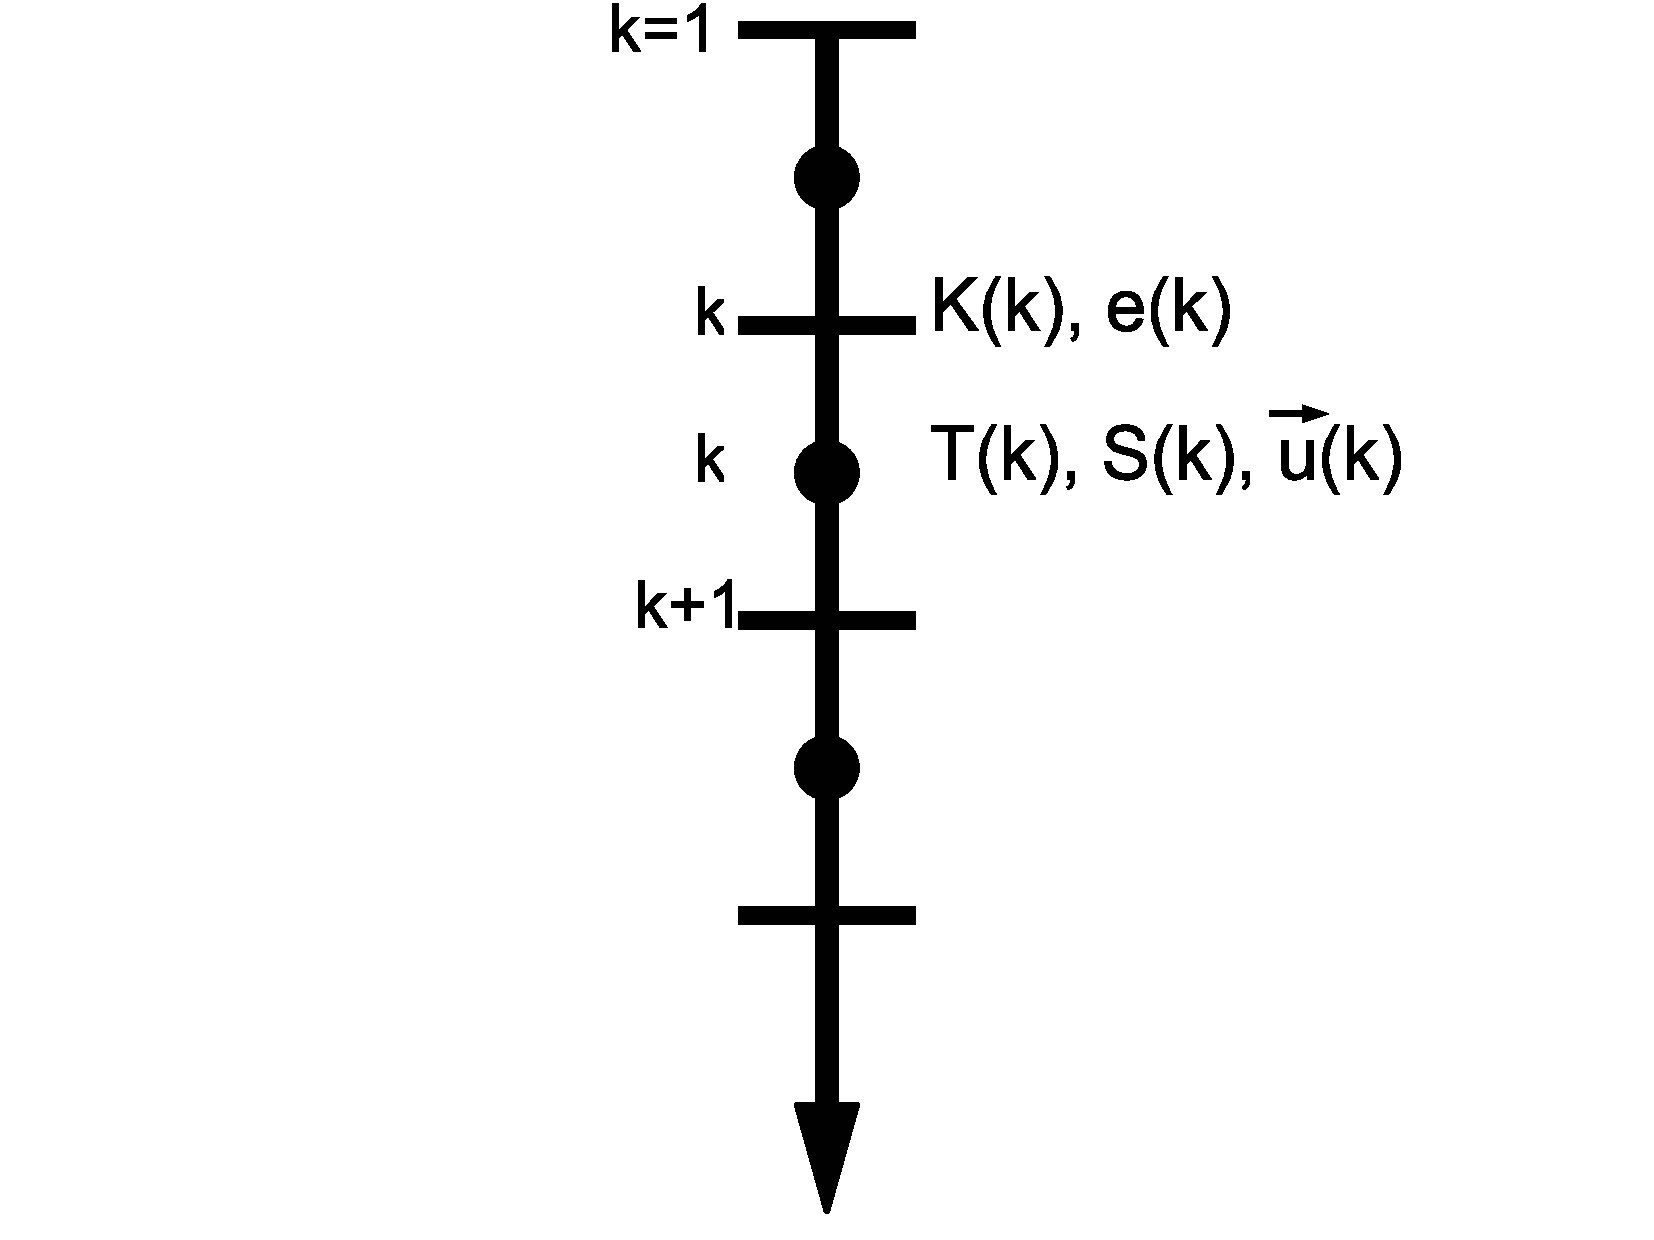
\includegraphics[height=14.5pc]{\EPSDIR/grille1D.pdf}
\caption{Vertical grid description of the 1D oceanic model from Gaspar et al. (1990) %\citet{gas90b}
.  \label{grille1}}
\end{figure}

To take into account the bathymetry effects on the oceanic vertical mixing, we introduced a bathymetry index (as the sea-land mask) which is worth 0 for free sea and 1 for levels under the sea-bed. For the vertical levels which have a bathymetry index equal to 1, we impose the prognostic variables values equal to the last free-sea level values. The 1D model thus does not carry out any energy transfer towards or coming from the bottom. Only the energy contained in the higher free levels is taken into account. 

We also introduced a diagnosis of mixed layer depth. The mixed layer base is diagnosed with an arbitrary criterion on the density profile: we assume that the thermocline corresponds to the vertical level for which the seawater density is superior to a 0.02 kg m$^{-3}$ variations compared to the density for a reference level (taken at 5m depth).  

Finally, the oceanic model must be initialized in temperature, salinity and current either from an oceanic analysis or from climatologies. 
%%%%%%%%%%%%%%%%%%%%%%%%%%%%%%%%%%%%%%%%%%%%%%%%%%%%%%%%%%%%%%%%%%%%%%%%%%%%%%
\clearpage


%\section{Inland water: Flake model}

%plm
%%%%%%%%%%%%%%%%%%%%%%%%%%%%%%%%%%%%%%%%%%%%%%%%%%%%%%%%%%%%%%%%%%%%%%%%%
%% 
%% Parameterization of Lakes in Numerical Weather Prediction.
%% Description of a Lake Model.
%% by DM
%% COSMO Technical Report No. 11 
%% 
%%%%%%%%%%%%%%%%%%%%%%%%%%%%%%%%%%%%%%%%%%%%%%%%%%%%%%%%%%%%%%%%%%%%%%%%%

%%%%%%%%%%%%%%%%%%%%%%%%%%%%%%%%%%%%%%%%%%%%%%%%%%%%%%%%%%%%%%%%%%%%%%%%%
%% Newcommands for refs
% \input{$HOME/LaTeX/jrn4rfs.incl_tex}
\newcommand{\ag}[3]{{\it Adv.\ Geophys.}, {\bf #1}, #2--#3.}\vspace{-1.4mm}
\newcommand{\arfm}[3]{{\it Ann.\ Rev.\ Fluid Mech.},\ {\bf #1},\ #2--#3.}
\newcommand{\asj}[3]{{\it Astrophys.\ J.},\ {\bf #1},\ #2--#3.}\vspace{-1.4mm}
\newcommand{\ao}[3]{{\it Atmosphere-Ocean},\ {\bf #1},\ #2--#3.}\vspace{-1.4mm}
\newcommand{\bamso}[3]{{\it Bull.\ Amer.\ Met.\ Soc.},\ {\bf #1},\ #2--#3.}\vspace{-1.4mm}
\newcommand{\blm}[3]{{\it Boundary-Layer Meteorol.},\ {\bf #1},\ #2--#3.}\vspace{-1.4mm}
\newcommand{\bpa}[3]{{\it Beitr.\ Phys.\ Atmosph.},\ {\bf #1},\ #2--#3.}\vspace{-1.4mm}
\newcommand{\cldyn}[3]{{\it Clim.\ Dynam.},\ {\bf #1},\ #2--#3.}\vspace{-1.4mm}
\newcommand{\crst}[3]{{\it Cold.\ Reg.\ Sci.\ Technol.},\ {\bf #1},\ #2--#3.}\vspace{-1.4mm}
\newcommand{\dan}[3]{{\it Dokl.\ Akad.\ Nauk SSSR.},\ {\bf #1},\ #2--#3.}\vspace{-1.4mm}
\newcommand{\dao}[3]{{\it Dyn.\ Atmos.\ Oceans},\ {\bf #1},\ #2--#3.}\vspace{-1.4mm}
\newcommand{\dsr}[3]{{\it Deep-Sea Res.},\ {\bf #1},\ #2--#3.}\vspace{-1.4mm}
\newcommand{\ems}[3]{{\it Environ.\ Modell.\ Softw.},\ {\bf #1},\ #2--#3.}\vspace{-1.4mm}
\newcommand{\fao}[3]{{\it Izv.\ Akad.\ Nauk SSSR. Fizika Atmosfery i Okeana},\ {\bf #1},\ #2--#3.}\vspace{-1.4mm}
\newcommand{\gfd}[3]{{\it Geophys.\ Fluid Dyn.},\ {\bf #1},\ #2--#3.}\vspace{-1.4mm}
\newcommand{\jam}[3]{{\it J.\ Appl.\ Meteorol.},\ {\bf #1},\ #2--#3.}\vspace{-1.4mm}
\newcommand{\jas}[3]{{\it J.\ Atmos.\ Sci.},\ {\bf #1},\ #2--#3.}\vspace{-1.4mm}
\newcommand{\jcli}[3]{{\it J.\ Climate},\ {\bf #1},\ #2--#3.}\vspace{-1.4mm}
\newcommand{\jcp}[3]{{\it J.\ Comput.\ Phys.},\ {\bf #1},\ #2--#3.}\vspace{-1.4mm}
\newcommand{\jcg}[3]{{\it J.\ Crystal Growth},\ {\bf #1},\ #2--#3.}\vspace{-1.4mm}
\newcommand{\jfe}[3]{{\it J.\ Fluid Eng.},\ {\bf #1},\ #2--#3.}\vspace{-1.4mm}
\newcommand{\jfm}[3]{{\it J.\ Fluid Mech.},\ {\bf #1},\ #2--#3.}\vspace{-1.4mm}
\newcommand{\jgr}[3]{{\it J.\ Geophys.\ Res.},\ {\bf #1},\ #2--#3.}\vspace{-1.4mm}
\newcommand{\jgrnew}[4]{{\it J.\ Geophys.\ Res.}, {\bf #1}(#2), #3, #4.}\vspace{-1.4mm}
\newcommand{\jhy}[3]{{\it J.\ Hydrometeorology}, {\bf #1}, #2--#3.}\vspace{-1.4mm}
\newcommand{\jmr}[3]{{\it J.\ Marine Res.},\ {\bf #1},\ #2--#3.}\vspace{-1.4mm}
\newcommand{\jplr}[3]{{\it J.\ Plankton Res.},\ {\bf #1},\ #2--#3.}\vspace{-1.4mm}
\newcommand{\jpo}[3]{{\it J.\ Phys.\ Oceanogr.},\ {\bf #1},\ #2--#3.}\vspace{-1.4mm}
\newcommand{\jweia}[3]{{\it J.\ Wind End.\ Industr.\ Aerodyn.},\ {\bf #1},\ #2--#3.}\vspace{-1.4mm}
\newcommand{\lio}[3]{{\it Limnol.\ Oceanogr.},\ {\bf #1},\ #2--#3.}\vspace{-1.4mm}
\newcommand{\loc}[3]{{\it Limnology and Oceanography}, {\bf #1},\ #2--#3.}\vspace{-1.4mm}
\newcommand{\mwr}[3]{{\it Mon.\ Weather Rev.},\ {\bf #1},\ #2--#3.}\vspace{-1.4mm}
\newcommand{\nat}[3]{{\it Nature},\ {\bf #1},\ #2--#3.}\vspace{-1.4mm}
\newcommand{\noh}[3]{{\it Nordic Hydrology},\ {\bf #1},\ #2--#3.}\vspace{-1.4mm}
\newcommand{\phf}[3]{{\it Phys.\ Fluids},\ {\bf #1},\ #2--#3.}\vspace{-1.4mm}
\newcommand{\po}[3]{{\it Prog.\ Oceanogr.},\ {\bf #1},\ #2--#3.}\vspace{-1.4mm}
\newcommand{\qj}[3]{{\it Quart.\ J.\ Roy.\ Meteorol.\ Soc.},\ {\bf #1},\ #2--#3.}\vspace{-1.4mm}
\newcommand{\rg}[3]{{\it Rev.\ Geophys.},\ {\bf #1},\ #2--#3.}\vspace{-1.4mm}
\newcommand{\rgsp}[3]{{\it Rev.\ Geophys.\ Space Phys.},\ {\bf #1},\ #2--#3.}\vspace{-1.4mm}
\newcommand{\sci}[3]{{\it Science},\ {\bf #1},\ #2--#3.}\vspace{-1.4mm}
\newcommand{\tel}[3]{{\it Tellus},\ {\bf #1},\ #2--#3.}\vspace{-1.4mm}
\newcommand{\vivl}[3]{{\it Verh.\ Internat.\ Ver.\ Limnol.},\ {\bf #1},\ #2--#3.}\vspace{-1.4mm}
\newcommand{\wrr}[3]{{\it Water Resour.\ Res.},\ {\bf #1},\ #2--#3.}\vspace{-1.4mm}
\newcommand{\wea}[3]{{\it Weather},\ {\bf #1},\ #2--#3.}\vspace{-1.4mm}
%% Useful newcommands
%\newcommand{\etal}{{et al.\ }}
% \newcommand{\eg}{{e.g.\ }}
% \newcommand{\ie}{{i.e.\ }}
% \newcommand{\para}{ }
% \newcommand{\pa}{\\}
% \newcommand{\tabline}{\hline}
%\newcommand{\beq}[1]{\begin{eqnarray}\label{{#1}}}
%\newcommand{\beq}{\begin{eqnarray}}
%\newcommand{\eeq}{\end{eqnarray}}
\newcommand{\beqn}{\begin{eqnarray*}}
\newcommand{\eeqn}{\end{eqnarray*}}
%%%%%%%%%%%%%%%%%%%%%%%%%%%%%%%%%%%%%%%%%%%%%%%%%%%%%%%%%%%%%%%%%%%%%%%%%

%\newpage

\section{Inland Water: Lake Model FLake}

\nopagebreak 
%
\noindent
In this section, a lake model (parameterisation scheme) capable of predicting the temperature structure
of lakes of various depth on time scales from a few hours to many years is presented.
A detailed description of the model, termed FLake, is given in Mironov (2010).
FLake is an integral (bulk) model.
It is based on a two-layer parametric representation of the evolving temperature profile within the water column
and on the integral energy budget for these layers.
The structure of the stratified layer between the upper mixed layer and the basin bottom, the lake thermocline,
is described using the concept of self-similarity (assumed shape) of the temperature-depth curve.
The same concept is used to describe the temperature structure
of the thermally-active upper layer of bottom sediments and of the ice and snow cover.
An entrainment equation for the depth of a convectively-mixed layer
and a relaxation-type equation for the depth of a wind-mixed layer
in stable and neutral stratification are developed
on the basis of the turbulence kinetic energy (TKE) equation integrated over the mixed layer.
Both mixing regimes are treated with due regard for the volumetric character of solar radiation heating.
Simple thermodynamic arguments are invoked to develop the evolution equations for the ice and snow depths.
The system of ordinary differential equations for the time-dependent prognostic quantities
that characterise the evolving temperature profile, see Figs.~\ref{ftr_T_sch_2media} and \ref{ftr_T_sch_4media}, is closed with algebraic (or transcendental) equations for diagnostic quantities,
such as the heat flux through the lake bottom and the equilibrium mixed-layer depth in stable or neutral stratification.

The resulting lake model is computationally very efficient but still incorporates much of the essential physics.

Within FLake, the lake water is treated as a Boussinesq fluid, i.e. the water density is taken to be constant equal
to the reference density except when it enters the buoyancy term in the TKE equation and the expression for the buoyancy frequency.

The other thermodynamic parameters are considered constant except for the snow density and the snow heat conductivity.

%
\begin{figure} %[h]
\begin{center}
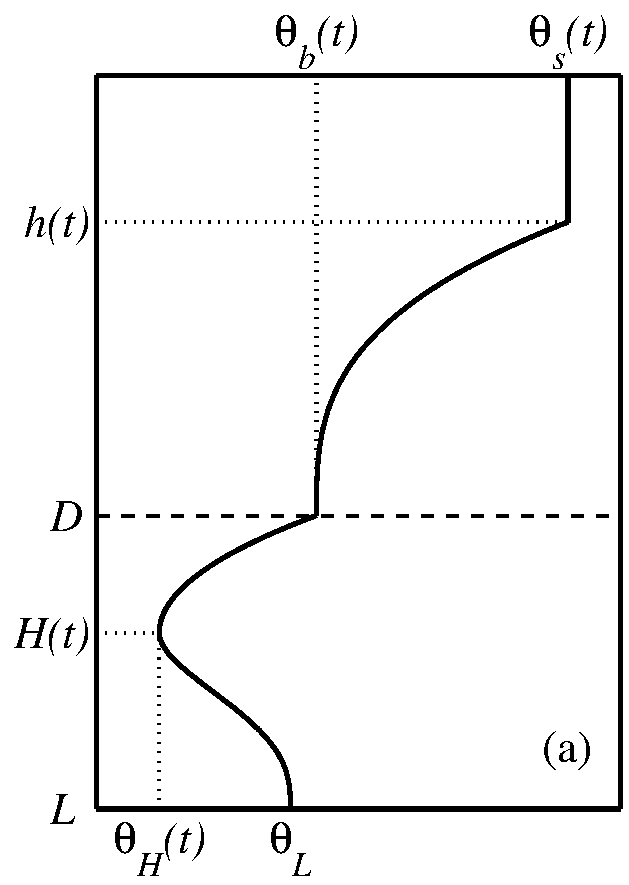
\includegraphics[width=11.5cm]{\EPSDIR/f_T_z_MLTBS_A_flk.pdf}
\begin{minipage}{0.9\textwidth}
\caption{Schematic representation of the temperature profile
in the mixed layer, in the thermocline, 
and in the thermally active layer of bottom sediments.
The evolving temperature profile is specified by several time-dependent quantities. 
These are 
the mixed-layer temperature $\theta_s(t)$ and its depth $h(t)$,
the temperature $\theta_b(t)$ at the water-bottom sediment interface,
the shape factor $C_{\theta}(t)$ with respect to the temperature profile in the thermocline,
the temperature $\theta_H(t)$ at the lower boundary of the upper layer of bottom sediments
penetrated by the thermal wave, and the depth $H(t)$ of that layer.
The temperature $\theta_{L}$ at the outer edge $z=L$
of the thermally active layer of bottom sediments is constant.}
\label{ftr_T_sch_2media}
\end{minipage}
\end{center}
\end{figure}
%
%
\begin{figure} %[h]
\begin{center}
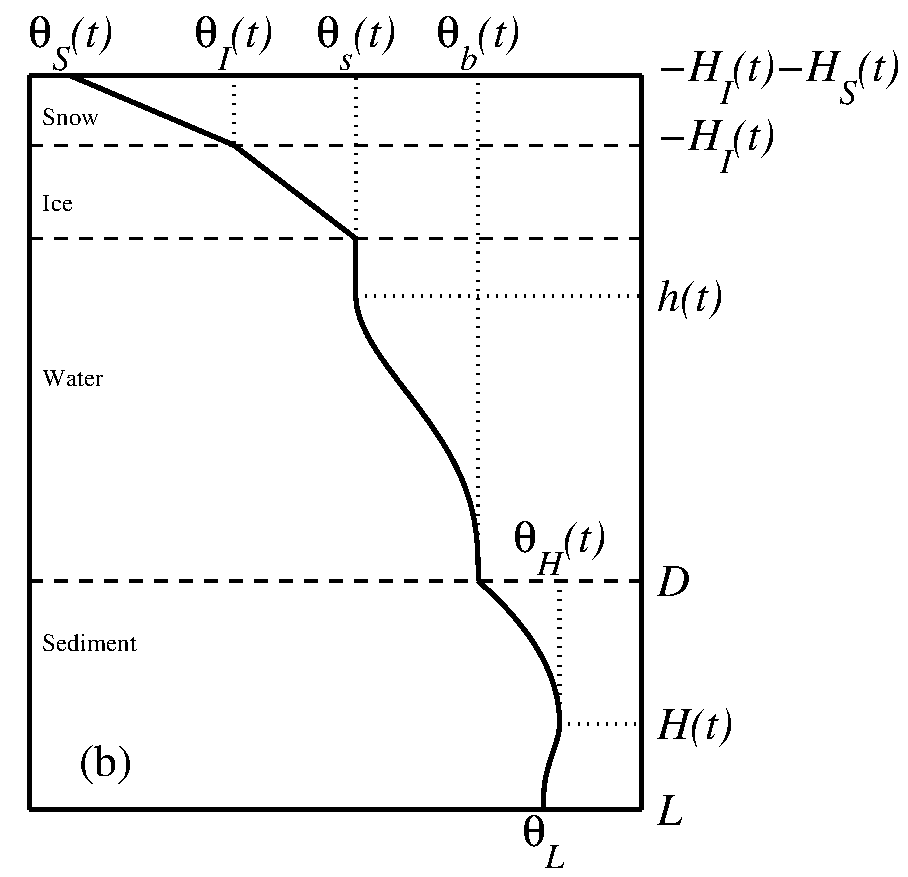
\includegraphics[width=15.0cm]{\EPSDIR/f_T_z_ISMLTBS_B_flk.pdf}
\begin{minipage}{0.9\textwidth}
\caption{
Apart from $\theta_s(t)$, $h(t)$, $\theta_b(t)$, $C_{\theta}(t)$, $\theta_H(t)$, and $H(t)$   
(see Fig.~\ref{ftr_T_sch_2media}), 
four additional quantities are computed in case the lake is covered by ice and snow. 
These are 
the temperature $\theta_S(t)$ at the air-snow interface,
the temperature $\theta_I(t)$ at the snow-ice interface,
the snow depth $H_S(t)$, and the ice depth $H_I(t)$.}
\label{ftr_T_sch_4media}
\end{minipage}
\end{center}
\end{figure}
%


\subsection{Equation of State}\label{eqstate}
\nopagebreak 
%
\noindent
We utilise the quadratic equation of state of the fresh water, 
%
\beq\label{eqstate2}
\rho_w = \rho_r\left[1-\frac{1}{2}a_T
\left(\theta-\theta_r\right)^2 \right] ,
\eeq
%
where $\rho_w$ is the water density, 
$\rho_r=999.98\approx1.0\cdot10^3$~kg$\cdot$m$^{-3}$ is the maximum density 
of the fresh water at the temperature $\theta_r=277.13$~K, 
and $a_T=1.6509\cdot 10^{-5}$~K$^{-2}$ is an empirical 
coefficient (Farmer and Carmack (1981)\nocite{farmer1981}). 
Equation (\ref{eqstate2}) is the simplest equation of state that 
accounts for the fact that the temperature of maximum density of 
the fresh water exceeds its freezing point 
$\theta_f=273.15$~K. 
According to Eq.~(\ref{eqstate2}), 
the thermal expansion coefficient 
$\alpha_T$ and the buoyancy parameter $\beta$ 
depend on the water temperature, 
%
\beq\label{buopar}
\beta(\theta) = g\alpha_T(\theta) = ga_T(\theta-\theta_r) ,
\eeq
%
where $g=9.81$~m$\cdot$s$^{-2}$ is the acceleration due to gravity.


\subsection{The Water Temperature}\label{wattem}
\nopagebreak 
%
\subsubsection{Parameterization of the Temperature Profile 
and the Heat Budget}\label{heatbudg_WC}
\nopagebreak 
%
\noindent
We adopt the following two-layer parameterization of the vertical temperature profile: 
%
\beq\label{Tprof_ML_T}
\theta = \left\{
\begin{array}{lll}
 \theta_s & \; \; \; \; \mbox{at} & \; \; 0\leq z\leq h \\ 
 \theta_s - (\theta_s-\theta_b)\Phi_{\theta}(\zeta) & 
\; \; \; \; \mbox{at} & \; \; h \leq z \leq D , 
\end{array}
\right.
\eeq
%
where 
$\Phi_{\theta}\equiv\left(\theta_s-\theta\right)/\left(\theta_s-\theta_b\right)$
is a dimensionless function of dimensionless depth 
\linebreak[4]
$\zeta\equiv\left(z-h\right)/\left(D-h\right)$.
The thermocline extends from the mixed-layer outer edge $z=h$ to the basin bottom $z=D$. Hereinafter the arguments of functions dependent on time and depth are not indicated (cf. Figs. \ref{ftr_T_sch_2media} and \ref{ftr_T_sch_4media} ). 

According to Eq.~(\ref{Tprof_ML_T}), 
$h$, $D$, $\theta_s$, $\theta_b$, and the mean temperature of the water column, 
\mbox{$\overline{\theta}\equiv D^{-1}\int_0^D\theta dz$}, 
are related through 
%
\beq\label{TemDepth_Rel} 
\overline{\theta} = \theta_s - C_{\theta}(1-h/D)(\theta_s-\theta_b) , 
\eeq
%
where 
%
\beq\label{ShapeFac_T} 
C_{\theta} = \int_0^1 \Phi_{\theta}(\zeta)d\zeta   
\eeq
%
is the shape factor. 

The parameterization of the temperature profile (\ref{Tprof_ML_T})
should satisfy the heat transfer equation
%
\beq\label{HTrans_eq}
\frac{\partial}{\partial t}(\rho c \theta) =
- \frac{\partial}{\partial z} (Q+I) ,
\eeq
%
where $Q$ is the vertical turbulent heat flux,
and $I$ is the heat flux due to solar radiation.

Integrating Eq.~(\ref{HTrans_eq}) over $z$ from 0 to $D$
yields the equation of the total heat budget, 
%
\beq\label{Tbdg_0-D}
D\frac{d\overline{\theta}}{dt} =
\frac{1}{\rho_w c_w}\left[ Q_s+I_s-Q_b-I(D) \right] , 
\eeq
%
where $c_w$ is the specific heat of water,
$Q_s$ and $I_s$ are the values of $Q$ and $I$, respectively, at the lake surface,
and $Q_b$ is the heat flux through the lake bottom.
The radiation heat flux $I_s$ that penetrates into the water 
is the surface value of the incident solar radiation flux
from the atmosphere multiplied by $1-\alpha_w$,
$\alpha_w$ being the albedo of the water surface with respect to solar radiation.
The surface flux $Q_s$ is a sum of the sensible and latent heat fluxes 
and the net heat flux due to long-wave radiation at the air-water interface.
%%
% It is a rather sophisticated function of the surface air layer parameters,
% of cloudiness and of the surface temperature. 
%%

Integrating Eq.~(\ref{HTrans_eq}) over $z$ from 0 to $h$
yields the equation of the heat budget in the mixed layer,
%
\beq\label{Tbdg_0-h}
h\frac{d\theta_s}{dt} =
\frac{1}{\rho_w c_w}\left[ 
Q_s+I_s-Q_h-I(h) \right] , 
\eeq
%
where $Q_h$ is the heat flux at the bottom of the mixed layer. 

Given the surface fluxes $Q_s$ and $I_s$ 
(these are delivered by the driving atmospheric model 
or are known from observations), 
and the decay law for the flux of solar radiation
, 
Eqs.~(\ref{TemDepth_Rel}), (\ref{Tbdg_0-D}) and (\ref{Tbdg_0-h}) 
contain seven unknowns, namely, 
$h$, $\overline{\theta}$, $\theta_s$, $\theta_b$, $Q_h$, $Q_b$ and $C_{\theta}$.
The mixed layer depth, the bottom heat flux and the shape factor  
are considered in what follows. 
One more relation is required.
Following Filyushkin and Miropolsky (1981)\nocite{filyushkin1981}, 
Tamsalu \etal (1997)\nocite{tamsalu1997} and Tamsalu and Myrberg (1998)\nocite{tamsalu1998}, 
we assume that in case of the mixed layer deepening, $dh/dt>0$, 
the profile of the vertical turbulent heat flux in the thermocline 
can be represented in a self-similar form. That is  
%
\beq\label{Qprof_T}
Q = Q_h - (Q_h-Q_b)\Phi_Q(\zeta) 
\; \; \; \; \; \; \mbox{at}  \; \; h\leq z\leq D ,
\eeq
%
where the shape function $\Phi_Q$ satisfies 
the boundary conditions $\Phi_Q(0)=0$ and $\Phi_Q(1)=1$.
Equation~(\ref{Qprof_T}) is suggested by
the travelling wave-type solution to the heat transfer equation.
If the mixed layer and the thermocline develop on the background
of a deep stably or neutrally stratified quiescent layer 
(this situation is encountered in the ocean and in the atmosphere),
the travelling wave-type solution shows
that both the temperature profile and the profile of the turbulent
heat flux are described by the same shape function,
\ie $\Phi_{\theta}(\zeta)=\Phi_Q(\zeta)$. 
In lakes, the thermocline usually extends from the bottom of the mixed layer
down to the basin bottom (except for very deep lakes). In this case, 
the travelling wave-type solution to the heat transfer equation
also suggests self-similar profiles of the temperature and of the heat flux,
however the relation between the shape functions $\Phi_{\theta}(\zeta)$ and $\Phi_Q(\zeta)$
is different. The issue is considered in Mironov (2008)\nocite{mironov2008}.

Integrating Eq.~(\ref{HTrans_eq})
with due regard for Eqs.~(\ref{Tprof_ML_T}) and (\ref{Qprof_T})
over $z'$ from $h$ to $z>h$,
then integrating the resulting expression 
over $z$ from $h$ to $D$, we obtain 
%
\beqn
\frac{1}{2}(D-h)^2\frac{d\theta_s}{dt} 
- \frac{d}{dt}\left[C_{\theta\theta}(D-h)^2(\theta_s-\theta_b)\right] =
\eeqn
%
\beq\label{Tb_dhdt_gt_0}
\frac{1}{\rho_w c_w}\left[C_Q(D-h)(Q_h-Q_b) + 
(D-h)I(h) - \int_h^D I(z)dz \right] ,
\eeq
%
where 
%
\beq\label{ShapeFac_Q} 
C_Q = \int_0^1\Phi_Q(\zeta)d\zeta   
\eeq
%
is the shape factor with respect to the heat flux, and
%
\beq\label{ShapeFac_T-2_def} 
C_{\theta\theta} = \int_0^1d\zeta\int_0^{\zeta'} \Phi_{\theta}(\zeta')d\zeta'   
\eeq
%
is the dimensionless parameter. 
The analysis in Mironov (2008) suggests that $C_Q=2C_{\theta\theta}/C_{\theta}$. 

In case of the mixed-layer stationary state or retreat, 
$dh/dt\le0$, Eq.~(\ref{Qprof_T}) is not justified. 
Then, the bottom temperature is assumed to be ``frozen'', 
%
\beq\label{Tb_dhdt_le_0}
\frac{d\theta_b}{dt}=0 .
\eeq
%
If $h=D$, then $\theta_b=\theta_s=\overline{\theta}$ 
and the mean temperature is computed from Eq.~(\ref{Tbdg_0-D}). 


\subsubsection{The skin temperature module}
\nopagebreak 
%
\noindent
The objective of introducing a skin temperature was to simulate a surface temperature 
representative of the energy budget at the lake surface, where the total derivative of 
temperature is in balance with the diffusion of the temperature plus a heat source, due 
to the divergence of the net radiation flux at the surface. In this optional module, the 
thickness of the skin layer is assumed to be constant and equal to 1 mm. During a model 
time step, this new surface temperature is then used to compute the new surface heat fluxes 
in the atmosphere, the new thickness of the mixed layer and the new thermocline profile.

The 1D heat transfer of heat in the lake writes:

\beq\label{skin1}
\rho_w c_w \frac{d\theta}{dt}=\kappa_w \nabla{\theta} + {\it{F}}
\eeq

Where $\theta$ is the water temperature, $\rho_w$ and $c_w$ the water density and heat capacity respectively,
$\kappa_w$ is the water heat transfer conductivity and $F$ a source term.\\

For a lake, {\it{$F$}} can be simplified into the divergence of the solar radiation {\it{$I$}} 
neglecting the divergence of the longwave radiation, which is a common assumption. At the 
continuum scale, decomposing an instantaneous field into an average plus a fluctuation and 
applying the Reynolds averaging operator to eq. \ref{skin1} allows expressing the tendency of
temperature. In the vicinity of the viscous layer, the turbulent term is negligible when 
compared to the diffusion term. If, on top of that, an assumption of horizontal homogeneity 
is applied to a steady state, eq. \ref{skin1} can be transformed into 
leads to:

\beq\label{skin2}
\kappa_w \frac{\partial^{2} \theta}{\partial z^{2}} + \frac{\partial I}{\partial z} = 0
\eeq

where $I$, the solar radiation that penetrates the water up to depth $z$ follows a Beer-Lambert decay law 
depending depth $z$ and the extinction coefficient of radiation in the water $\epsilon$.

Equation \ref{skin2} can be integrated between the surface and the depth $h$ to give the 
expression of the skin temperature $\theta_{skin}$ as a function of $Q_s$, $I_s$, $\theta_s$ and depth $h$:

\begin{eqnarray}\label{skin3}
\theta_{skin} = \theta_{s} + \frac{h}{\kappa_w}\left[ Q_s+I_s\left(1-\frac{1-e^{-\epsilon h}}{\epsilon h} \right)\right] 
\end{eqnarray}

Details of the computation can be found in Le Moigne \etal (2016)\nocite{LeMoigne_2016}.


\subsubsection{The Mixed-Layer Depth}
\nopagebreak 
%
\noindent
Convective deepening of the mixed layer is described by the entrainment equation. 
This equation is conveniently formulated in terms of the dependence
of the so-called entrainment ratio $A$ on one or the other stratification parameter. 
The entrainment ratio is a measure of the entrainment efficiency.
It is commonly defined as a negative of the
ratio of the heat flux due to entrainment 
at the bottom of the mixed layer, $Q_h$, 
to an appropriate heat flux scale, $Q_*$. 
In case of convection driven by the surface flux,
where the forcing is confined to the boundary,
the surface heat flux $Q_s$ serves as an appropriate flux scale.
This leads to the now classical Deardorff (1970a, 1970b)\nocite{deardorff1970a,deardorff1970b} convective scaling,
where $h$ and $|h\beta Q_s/(\rho_w c_w)|^{1/3}$ 
serve as the scales of length and velocity, respectively. 

The Deardorff scaling is unsuitable for convective flows
affected by the solar radiation heating that is not 
confined to the boundary but is distributed over the water column.
If the mixed-layer temperature exceeds the temperature of maximum density,
convective motions are driven by surface cooling,
whereas radiation heating tends to stabilise the water column,
arresting the mixed layer deepening
(Soloviev (1979)\nocite{soloviev1979}; Mironov and Karlin (1989)\nocite{mironov1989}).
Such regime of convection is encountered in the oceanic upper layer 
(\eg Kraus and Rooth (1961)\nocite{kraus1961}, Soloviev and Vershinskii (1982)\nocite{soloviev1982}, Price \etal (1986)\nocite{price1986} 
and in fresh-water lakes (\eg Imberger (1985)\nocite{imberger1985}).
If the mixed-layer temperature is below that of maximum density,
volumetric radiation heating leads to de-stabilisation of
the water column and thereby drives convective motions.
Such regime of convection is encountered in fresh-water lakes in spring.
Convective mixing often occurs under the ice, 
when the snow cover overlying the ice vanishes and
solar radiation penetrates down through the ice 
(\eg Farmer (1975)\nocite{farmer1975}, Mironov and Terzhevik (2000)\nocite{mironov2000}, Mironov \etal (2002)\nocite{mironov2002}, Jonas \etal (2003)\nocite{jonas2003}).

In order to account for the vertically distributed character of 
the radiation heating,
we make use of a generalised convective heat flux scale 
%
\beq\label{Qconv_gener}
Q_* = Q_s + I_s +I(h) - 2h^{-1}\int_0^h I(z) dz ,
\eeq
%
and define the convective velocity scale and the entrainment ratio as 
%
\beq\label{Wconv_A-gener}
w_*=\left[-h\beta(\theta_s)Q_*/(\rho_w c_w)\right]^{1/3}, 
\; \; \; \; \; \; \; \; \; \; 
A=-Q_h/Q_*, 
\eeq
%
respectively.
In order to specify $A$, we employ the entrainment equation in the form 
%
\beq\label{EntrEq_2term}
A + \frac{C_{c2}}{w_*}\frac{dh}{dt} = C_{c1} ,
\eeq
%
where $C_{c1}$ and $C_{c2}$ are dimensionless constants 
(the estimates of these and other empirical constants of the model
are discussed in Section \ref{constempirrel} and summarised in the Appendix).
The second term on the l.h.s.\ of Eq.~(\ref{EntrEq_2term})
is the spin-up correction term introduced by Zilitinkevich (1975)\nocite{zilitin1975}.
This term prevents an unduly fast growth of $h$
when the mixed layer is shallow.
If the spin-up term is small, 
Eq.~(\ref{EntrEq_2term}) reduces to a simple relation $A=C_{c1}$ 
that proved to be a sufficiently accurate approximation 
for a large variety of geophysical and laboratory convective flows 
Zilitinkevich (1991)\nocite{zilitin1991}.

Equations~(\ref{Qconv_gener}), (\ref{Wconv_A-gener}) and (\ref{EntrEq_2term})
should be used to compute the mixed-layer depth
when the buoyancy flux $B_*=\beta(\theta_s)Q_*/(\rho_w c_w)$ is negative. 
The quantity $-hB_*\equiv w_*^3$ is a measure of the generation rate of 
the turbulence kinetic energy in a layer of depth $h$ by the buoyancy forces 
(see a discussion in Mironov \etal (2002)).
A negative $B_*$ indicates that the TKE is generated through convective instability.
Otherwise, the TKE is lost to work against the gravity. 
This occurs when the density stratification is stable.
A different formulation for the mixed-layer depth is then required.


 \ \\
\noindent
\nopagebreak
%
\noindent
Mironov \etal (1991)\nocite{mironovbook1991} used a diagnostic equation to determine
the wind-mixed layer depth in stable and neutral stratification.
That is, $h$ was assumed to adjust to external forcing 
on a time scale that does not exceed the model time step.
This assumption is fair if seasonal changes of temperature 
and mixing conditions are considered and the model time step is typically one day.  
The assumption is likely to be too crude to consider diurnal variations. 
To this end, We utilise a relaxation-type rate equation for the depth 
of a stably or neutrally stratified wind-mixed layer.
It reads 
%
\beq\label{h_SBL_relax}
\frac{dh}{dt} = \frac{h_e-h}{t_{rh}} . 
\eeq
%
Here, $h_e$ is the equilibrium mixed-layer depth,
and $t_{rh}$ is the relaxation time scale given by 
%
\beq\label{t_relax_SBL}
t_{rh} = \frac{h_e}{C_{rh}u_*} ,
\eeq
%
where $u_{*}=|\tau_s/\rho_w c_w|^{1/2}$ is the surface friction velocity, 
$\tau_s$ being the surface stress,
and $C_{rh}$ is a dimensionless constant.
A rate equation (\ref{h_SBL_relax})
with the relaxation time scale proportional to the 
reciprocal of the Coriolis parameter
[that is a particular case of Eq.~(\ref{t_relax_SBL}) 
with $h_e$ specified through Eq.~(\ref{he_SBL_ZM3term})]
was favourably tested by Zilitinkevich \etal (2002)\nocite{zilitin2002} and 
Zilitinkevich and Baklanov (2002)\nocite{zilitinbak2002} 
against data from atmospheric measurements
and was recommended for practical use.

In order to specify $h_e$, we make use of
a multi-limit formulation for the equilibrium depth of a stably
or neutrally stratified boundary layer proposed by Zilitinkevich and Mironov (1996)\nocite{zilitinmiro1996}.
Based on the analysis of the TKE budget,
these authors proposed a generalised equation for the equilibrium boundary-layer depth 
that accounts for the combined effects of rotation, surface buoyancy flux and
static stability at the boundary-layer outer edge [Eq.~(30) in op.~cit.].
That equation reduces to the equations proposed earlier by
Rossby and Montgomery (1935)\nocite{rossby1935}, Kitaigorodskii (1960)\nocite{Kitaigo1960}
and Kitaigorodskii and Joffre (1988)\nocite{kitaigo1988}
in the limiting cases of a truly neutral rotating boundary layer, 
the surface-flux-dominated boundary layer, 
and the imposed-stability-dominated boundary layer, respectively.
It also incorporates the Zilitinkevich (1972)\nocite{zilitin1972} and the Pollard \etal (1973)\nocite{pollard1973} 
equations that describe the intermediate regimes,
where the effects of rotations and stratification essentially interfere
and are roughly equally important.
We adopt a simplified version of the Zilitinkevich and Mironov (1996) equation
[Eq.~(26) in op.~cit.]
that does not incorporate the Zilitinkevich (1972) and the Pollard \etal (1973) scales.
It reads 
%
\beq\label{he_SBL_ZM3term}
\left( \frac{fh_e}{C_n u_*} \right)^2
+ \frac{h_e}{C_s L}
+ \frac{Nh_e}{C_i u_*}
= 1 ,
\eeq
%
where $f=2\Omega\sin\phi$ is the Coriolis parameter,
$\Omega=7.29\cdot10^{-5}$~s$^{-1}$ is the angular velocity of the earth's rotation,
$\phi$ is the geographical latitude,
$L$ is the Obukhov length,
$N$ is the buoyancy frequency below the mixed layer,
and $C_n$, $C_s$ and $C_i$ are dimensionless constants.
A generalised  formulation for the Obukhov length is used, 
$L=u_*^3/(\beta Q_*/\rho_w c_w)$,
that accounts for the vertically distributed character of the solar radiation heating
(note that the von K\'arm\'an constant is not included into the definition of $L$).
A mean-square buoyancy frequency in the thermocline,
$\overline{N}=\left[(D-h)^{-1}\int_h^DN^2dz\right]^{1/2}$,
is used as an estimate of $N$ in Eq.~(\ref{he_SBL_ZM3term}).

One further comment is in order.
Zilitinkevich \etal (2002) reconsidered the problem of 
the equilibrium stable boundary-layer depth.
They concluded that the Zilitinkevich (1972) scale, 
$|u_*L/f|^{1/2}$, and the Pollard \etal (1973) scale,
$u_*/|Nf|^{1/2}$, are the appropriate depth scales for the 
boundary layers dominated by the surface buoyancy flux
and by the static stability at the boundary-layer outer edge, respectively.
In other words, $h_e$ depends on the Coriolis parameter 
no matter how strong the static stability.
This is different from Eq.~(\ref{he_SBL_ZM3term})
where the limiting scales are $L$ and $u_*/N$, respectively.
The problem was further examined by Mironov and Fedorovich (2010)\nocite{mironovfedo2010}.
They showed that the above scales are particular cases of more general power-law formulations,
namely, $h/L\propto (|f|L/u_*)^{-p}$ and $hN/u_*\propto (|f|/N)^{-q}$ for the 
boundary layers dominated by the surface buoyancy flux 
and by the static stability at the boundary-layer outer edge,
respectively. The Zilitinkevich (1972) and Pollard \etal (1973) scales 
are recovered with $p=1/2$ and $q=1/2$, 
whereas the Kitaigorodskii (1960) and Kitaigorodskii and Joffre (1988) 
are recovered with $p=0$ and $q=0$. 
Scaling arguments are not sufficient to fix the exponents $p$ and $q$.
They should be evaluated on the basis of experimental data.
Available data from observations and from large-eddy simulations are uncertain.
They do not make it possible to evaluate $p$ and $q$ to sufficient accuracy 
and to conclusively decide between the alternative formulations for the boundary-layer depth.
Leaving the evaluation of $p$ and $q$ for future studies, we utilise Eq.~(\ref{he_SBL_ZM3term}).
This simple interpolation formula is consistent with the complexity of the present lake model
and is expected to be a sufficiently accurate approximation for most practical purposes.

One more limitation on the equilibrium mixed-layer depth should be taken into account.
Consider the situation where
the mixed-layer temperature exceeds the temperature of maximum density,
the surface flux $Q_s$ is negative, whereas  
the heat flux scale $Q_*$ given by Eq.~(\ref{Qconv_gener}) is positive 
(this can take place if $-Q_s/I_s<1$).
A positive $Q_*$ indicates the the mixed layer of depth $h$ 
is statically stable. 
A negative $Q_s$, however, indicates that convective instability 
should take place, leading to the development of a convectively mixed layer 
whose deepening is arrested by the solar radiation heating.
The equilibrium depth $h_c$ of such mixed layer is given by
(see \eg Mironov and Karlin (1989)) 
%
\beq\label{he_CBL_Qstar}
Q_*(h_c) = Q_s + I_s +I(h_c) - 2h_c^{-1}\int_0^{h_c} I(z) dz = 0 .
\eeq
%
This regime of convection is encountered on calm sunny days.
If the wind suddenly ceases, Eq.~(\ref{he_SBL_ZM3term}) predicts a very shallow
stably-stratified equilibrium mixed layer to which the mixed layer  
of depth $h>h_e$ should relax.
In fact, however, the mixed layer would relax towards a convectively mixed layer
whose equilibrium depth is given by Eq.~(\ref{he_CBL_Qstar}).
In order to account for this constraint, 
we require that $h_e\ge h_c$ if $Q_*(h)>0$ and $\theta_s>\theta_r$. 


\subsection{The Water--Bottom Sediment Interaction}\label{watbotinter}
\nopagebreak 
%
\paragraph{Parameterization of the Temperature Profile 
and the Heat Budget}\label{heatbudg_BS}
\nopagebreak
%
\noindent
We adopt the following two-layer parametric representation,
of the evolving temperature profile in 
the thermally active layer of bottom sediments 
proposed by Golosov \etal (1998)\nocite{golosov1998}:

\beq\label{TProfPar_BS}
\theta = \left\{ 
\begin{array}{lll}
\theta_b -\left[\theta_b-\theta_H\right]\Phi_{B1}(\zeta_{B1})  & 
\; \; \; \; \mbox{at}  & \; \; D\leq z \leq H \\ 
\theta_H - \left[\theta_H-\theta_L\right]\Phi_{B2}(\zeta_{B2}) & 
\; \; \; \; \mbox{at}  & \; \; H\leq z \leq L , 
\end{array}
\right.
\eeq
Where, $\theta_{L}$ is the (constant) temperature at the outer edge $z=L$ 
of the thermally active layer of the sediments, 
$\theta_{H}$ is the temperature at the depth $H$ 
where the vertical temperature gradient is zero, 
and $\Phi_{B1}\equiv (\theta_b-\theta)/(\theta_b-\theta_H)$ and 
$\Phi_{B2}\equiv (\theta_H-\theta)/(\theta_H-\theta_L)$ 
are dimensionless functions of dimensionless depths 
$\zeta_{B1}\equiv (z-D)/(H-D)$ and $\zeta_{B2}\equiv (z-H)/(L-H)$, respectively.

The parameterization (\ref{TProfPar_BS}) 
should satisfy the heat transfer equation (\ref{HTrans_eq}),
where the heat flux $Q$ is due to molecular heat conduction 
and the bottom sediments are opaque to radiation.
Integrating Eq.~(\ref{HTrans_eq}) over $z$
from $z=D$ to $z=H$ 
with due regard for Eq.~(\ref{TProfPar_BS}),
we obtain 
%
\beq\label{HBal_BS-D_H}
\frac{d}{dt} \left[(H-D)\theta_b-C_{B1}(H-D)(\theta_b-\theta_H)\right]
-\theta_H\frac{dH}{dt}
= \frac{1}{\rho_wc_w}\left[Q_b+I(D)\right] ,
\eeq
%
where the heat flux at $z=H$ is zero by virtue of 
the zero temperature gradient there.

Integrating Eq.~(\ref{HTrans_eq}) over $z$ from $z=H$ to $z=L$,
we obtain 
%
\beq\label{HBal_BS-H_L}
\frac{d}{dt} \left[(L-H)\theta_H-C_{B2}(L-H)(\theta_H-\theta_L)\right]
+\theta_H\frac{dH}{dt} = 0 ,
\eeq
%
where the heat flux at $z=L$ (the geothermal heat flux) is neglected.

The shape factors $C_{B1}$ and $C_{B2}$ are given by
%
\beq\label{BS_shape_fact}
C_{B1} = \int_0^1 \Phi_{B1}(\zeta_{B1}) d \zeta_{B1} ,
\; \; \; \; \; \;
C_{B2} = \int_0^1 \Phi_{B2}(\zeta_{B2}) d \zeta_{B2} .
\eeq
%


\paragraph{Heat Flux through the Bottom}\label{heatflux_BS}
\nopagebreak
%
\noindent
The bottom heat flux $Q_b$ is due to molecular heat conduction through 
the uppermost layer of bottom sediments. It can be estimated 
as the product of the negative of the temperature gradient at $z=D+0$
and the molecular heat conductivity. 
The uppermost layer of bottom sediments is saturated with water.
Its water content typically exceeds 90\% and its physical properties,
including the heat conductivity, 
are very close to the properties of the lake water. 
Then, the heat flux through the lake bottom is given by 
%
\beq\label{HFlux_bottom}
Q_b = - \kappa_w \frac{\theta_H-\theta_b}{H-D} \Phi_{B1}'(0) ,
\eeq
%
where $\kappa_w$ is the molecular heat conductivity of water.
This relation closes the problem.

It should be stressed that Eqs.~(\ref{HBal_BS-D_H}), (\ref{HBal_BS-H_L})
and (\ref{HFlux_bottom}) do not contain 
the molecular heat conductivity of bottom sediments,
a quantity that is rarely known to a satisfactory degree of precision. 
It is through the use of the integral (bulk) approach,
based on the parameterization (\ref{TProfPar_BS}) of the temperature profile,
that the molecular heat conductivity of bottom sediments
is no longer needed.


\subsection{Ice and Snow Cover}\label{icesnow}
\nopagebreak
%
\noindent
In this section, a two-layer thermodynamic (no rheology) model 
of the ice and snow cover is described. 
It is based on a self-similar parametric representation of 
the temperature profile within ice and snow 
and on the integral heat budgets of the ice and snow layers. 
The approach is, therefore, conceptually similar to the approach 
used above to describe the temperature structure of the mixed layer, 
of the lake thermocline, and of the thermally active layer of bottom sediments. 
Notice that the assumption about the shape of the temperature profile within the ice, 
the simplest of which is the linear profile, 
is either explicit or implicit in a number of ice models developed to date. 
A model of ice growth based on a linear temperature distribution 
was proposed by Stefan as early as 1891. 


\paragraph{Parameterization of the Temperature Profile 
and the Heat Budget}\label{heatbudg_SI} 
\nopagebreak
%
\noindent
We adopt the following parametric representation of the evolving 
temperature profile within ice and snow: 
%
\beq\label{Tpro_ice_snow}
\theta = \left\{
\begin{array}{lll}
\theta_f - [\theta_f-\theta_I]\Phi_I(\zeta_I)  
& \; \; \; \; \mbox{at}  & \; \; -H_I \leq z \leq 0 \\
\theta_I - [\theta_I-\theta_S]\Phi_S(\zeta_S) 
& \; \; \; \; \mbox{at}  & \; \; -[H_I+H_S]\leq z \leq -H_I .
\end{array}
\right.
\eeq
%
Here, 
$z$ is the vertical co-ordinate (positive downward) 
with the origin at the ice-water interface, 
$H_I$ is the ice thickness, $H_S$ is the thickness of snow overlaying the ice, 
$\theta_f$ is the fresh-water freezing point, 
$\theta_I$ is the temperature at the snow-ice interface, 
and $\theta_S$ is the temperature at the air-snow interface. 
Notice that the freezing point of salt water is a decreasing function of salinity. 
A model that accounts for this dependence and is applicable to 
the ice over salt lakes or seas is presented by Mironov and Ritter (2004)\nocite{mironovritter2004}. 
Dimensionless universal functions 
$\Phi_I\equiv (\theta_f-\theta)/(\theta_f-\theta_I)$ and 
$\Phi_S\equiv (\theta_I-\theta)/(\theta_I-\theta_S)$ 
of dimensionless depths 
$\zeta_I\equiv -z/H_I$ and $\zeta_S\equiv -(z+H_I)/H_S$, respectively, 
satisfy the boundary conditions $\Phi_I(0)=0$, $\Phi_I(1)=1$, 
$\Phi_S(0)=0$, and $\Phi_S(1)=1$.

According to Eq.~(\ref{Tpro_ice_snow}), the heat fluxes 
through the ice, $Q_I$, and through the snow, $Q_S$, 
due to molecular heat conduction are given by 
%
\beq\label{HFl_ice_snow}
Q_I = - \kappa_i \frac{\theta_f-\theta_I}{H_I} \frac{d\Phi_I}{d\zeta_I} ,
\; \; \; \; \; \;
Q_S = - \kappa_s \frac{\theta_I-\theta_S}{H_S} \frac{d\Phi_S}{d\zeta_S},
\eeq
%
where $\kappa_i$ and $\kappa_s$ are the heat conductivities 
of ice and snow, respectively. 

The parameterization of the temperature profile (\ref{Tpro_ice_snow}) 
should satisfy the heat transfer equation (\ref{HTrans_eq}). 
Integrating Eq.~(\ref{HTrans_eq}) over $z$ 
from the air-snow interface $z=-(H_I+H_S)$ 
to just above the ice-water interface $z=-0$ 
with due regard for the parameterization (\ref{Tpro_ice_snow}),
we obtain the equation of the heat budget of the snow-ice cover,
%
\beqn
\frac{d}{dt} \{ \rho_i c_i H_I \left[\theta_f - C_{I}(\theta_f-\theta_I) \right]
+ \rho_s c_s H_S \left[\theta_I - C_{S}(\theta_I-\theta_S) \right] \}
- \rho_s c_s \theta_S \frac{d}{dt}(H_I+H_S) = 
\eeqn
\beq\label{HBal_0-Hs}
Q_s + I_s - I(0) + \kappa_i\frac{\theta_f-\theta_I}{H_I}\Phi_I'(0) .
\eeq
%
Here, $\rho_i$ and $\rho_s$ are the densities of ice and of snow, 
respectively, 
$c_i$ and $c_s$ are specific heats of these media, 
and $Q_s$ and $I_s$ are the values of $Q$ and $I$, respectively, 
at the air-snow or, if snow is absent, at the air-ice interface. 
The radiation heat flux $I_s$ that penetrates into the interior of snow-ice cover
is the surface value of the incident solar radiation flux 
from the atmosphere multiplied by $1-\alpha_i$, 
$\alpha_i$ being the albedo of the ice or snow surface with respect to solar radiation.
The dimensionless parameters $C_{I}$ and $C_{S}$, 
the shape factors, are given by  
%
\beq\label{SI_shape_fact}
C_{I} = \int_0^1 \Phi_I(\zeta_I) d \zeta_I ,
\; \; \; \; \; \;
C_{S} = \int_0^1 \Phi_S(\zeta_S) d \zeta_S .
\eeq
%

The heat flux at the snow-ice interface is assumed to be continuous,
that is
%
\beq\label{flux_match_Hi}
-\kappa_i\frac{\theta_f-\theta_I}{H_I}\Phi_I'(1) 
= -\kappa_s\frac{\theta_I-\theta_S}{H_S}\Phi_S'(0) .
\eeq
%

Equations~(\ref{HBal_0-Hs}) and (\ref{flux_match_Hi}) 
serve to determine temperatures at the air-snow and at the snow-ice interfaces,
when these temperatures are below the freezing point,
\ie when no melting at the snow surface (ice surface, when snow is absent) takes place.
During the snow (ice) melting from above, the temperatures $\theta_S$ and $\theta_I$
remain equal to the freezing point $\theta_{f}$,
and the heat fluxes $Q_S$ and $Q_I$ are zero.


\paragraph{Snow and Ice Thickness}\label{snowicethick_SI}
\nopagebreak
%
\noindent
The equations governing the evolution of the snow thickness and of the ice thickness
are derived from the heat transfer equation (\ref{HTrans_eq})
that incorporates an additional term on its right-hand side,
namely, the term $f_M(z)L_fdM/dt$ 
that describes the rate of heat re\-lease/con\-sump\-tion 
due to accretion/melting of snow and ice.
Here, $M$ is the mass of snow  or ice per unit area,
$L_f$ is the latent heat of fusion, and
$f_M(z)$ is a function that satisfies the normalization conditions
$\int_{H_I}^{H_I+H_S}f_M(z)dz=1$ and $\int_0^{H_I}f_M(z)dz=1$ 
for snow and ice, respectively. 

The accumulation of snow is not computed within the ice-snow model.
The rate of snow accumulation is assumed to be a known time-dependent quantity 
that is provided by the atmospheric model or is known from observations.  
Then, the evolution of the snow thickness during the snow accumulation
and no melting is computed from 
%
\beq\label{snow_accum}
\frac{d\rho_s H_S}{dt} = \left(\frac{dM_S}{dt}\right)_a ,
\eeq
%
where $M_S=\rho_s H_S$ is the snow mass per unit area,
and $(dM_S/dt)_a$ is the (given) rate of snow accumulation.

When the temperature $\theta_I$ at the upper surface of the ice
is below the freezing point $\theta_f$,
the heat conduction through the ice causes the ice growth.
This growth is accompanied by a release of heat at the lower surface of the ice
that occurs at a rate $L_fdM_I/dt$,
where $M_I=\rho_i H_I$ is the ice mass per unit area.
The normalization function $f_M$ is equal to zero throughout
the snow-ice cover except at the ice-water interface where
$f_M=\delta(0)$, $\delta(z)$ being the Dirac delta function.
Integrating Eq.~(\ref{HTrans_eq}) from $z=-0$ to $z=+0$
with due regard for this heat release yields the equation for the ice thickness. 
It reads
%
\beq\label{ice_growth}
L_f \frac{d\rho_i H_I}{dt} =
Q_w + \kappa_i\frac{\theta_f-\theta_I}{H_I}\Phi_I'(0) ,
\eeq
%
where $Q_w$ is the heat flux
in the near-surface water layer just beneath the ice.
If the r.h.s.\ of Eq.~(\ref{ice_growth}) is negative,
\ie the negative of the heat flux in the water, $Q_w$,
exceeds the negative of the heat flux in the ice, $Q_I|_{z=0}$,
ice ablation takes place.

As the atmosphere heats the snow surface,
the surface temperature eventually reaches the freezing point 
and the snow and ice melting sets in.
This process is accompanied by a consumption of heat 
at rates $L_fd\rho_sH_S/dt$ and $L_fd\rho_iH_I/dt$ for snow and ice, respectively.
Notice that the exact form of the normalization function $f_M$ is not required
by virtue of the normalization conditions considered above.
Integrating Eq.~(\ref{HTrans_eq}) from $z=-(H_I+H_S)-0$ to $z=-H_I$ 
with due regard for the heat loss due to snow melting
and adding the (given) rate of snow accumulation
yields the equation for the snow thickness,
%
\beq\label{snow_melt}
L_f \frac{d\rho_s H_S}{dt} = 
-(Q_s + I_s) + I(-H_I) 
+ L_f\left(\frac{dM_S}{dt}\right)_a + c_s\theta_fH_S\frac{d\rho_s}{dt} .
\eeq
%
Integrating Eq.~(\ref{HTrans_eq}) from $z=-H_I$ to $z=+0$
with due regard for the heat loss due to ice melting
yields the equation for the ice thickness,
%
\beq\label{ice_melt}
L_f \frac{d\rho_i H_I}{dt} =
Q_w + I(0) - I(-H_I) .
\eeq
%

If the ice melts out earlier than snow, 
the snow depth is instantaneously set to zero.


\paragraph{The Temperature Profile beneath the Ice}\label{Tbelowice}
\nopagebreak
%
\noindent
The simplest assumption is to keep the temperature profile unchanged 
over the entire period of ice cover. This assumption is fair for deep lakes, 
where the heat flux through the bottom is negligibly small. In shallow lakes, 
this assumption may lead to an underestimation of the mean temperature.
The heat accumulated in the thermally active upper layer of bottom sediments
during spring and summer is returned back to the water column during winter,
leading to an increase of the water temperature under the ice.
The water temperature under the ice can also increase due to heating 
by solar radiation penetrating down through the ice.
The thermodynamic regimes encountered in ice-covered lakes are many and varied.
Their detailed description requires a set of sophisticated parameterizations.
The use of such parameterizations in the framework of the present lake model is,
however, hardly justified. 
The point is that it is the snow (ice) surface temperature 
that communicates information to the atmosphere, the water temperature is not 
directly felt by the atmospheric surface layer.
It is, therefore, not vital that the temperature regimes in ice-covered lakes 
be described in great detail. Only their most salient features should be accounted for,
first of all, the heat budget of the water column. 

When the lake is ice-covered, the temperature at the ice-water interface 
is fixed at the freezing point $\theta_s=\theta_{f}$.
In case the bottom temperature is less than the temperature of maximum density,
$\theta_b<\theta_r$, the mixed-layer depth and the shape factor are
kept unchanged, $dh/dt=0$ and $dC_{\theta}/dt=0$,
the mean temperature $\overline{\theta}$ is computed
from Eq.~(\ref{Tbdg_0-D}) and the bottom temperature $\theta_b$ 
is computed from Eq.~(\ref{TemDepth_Rel}). 
If the entire water column appears to be mixed at the moment of freezing, 
\ie $h=D$ and $\theta_s=\overline{\theta}=\theta_b$, 
the mixed layer depth is reset to zero, $h=0$, 
and the shape factor is set to its minimum value, $C_{\theta}=0.5$ 
(see Section \ref{empir_shapefun}). 

The heat flux from water to ice is estimated from 
%
\beq\label{HFlux_water_ice_1}
Q_w = -{\kappa_w}\frac{\theta_b-\theta_s}{D} ,
\eeq
%
if $h=0$, and $Q_w=0$ otherwise.
Notice that the estimate of $Q_w$ given by Eq.~(\ref{HFlux_water_ice_1})
and the shape factor $C_{\theta}=0.5$ correspond to a linear 
temperature profile over the entire water column.
A linear profile is encountered in ice-covered shallow lakes when 
$\theta_b<\theta_r$ and the heat flux is from the bottom sediments to the lake water.

As the bottom temperature reaches the temperature of maximum density,
convection due to bottom heating sets in. To describe this regime of convection 
in detail, a convectively mixed layer whose temperature is close to $\theta_r$, 
and a thin layer adjacent to the bottom,
where the temperature decreases sharply from $\theta_b>\theta_r$ to $\theta_r$, 
should be thoroughly considered. 
We neglect these peculiarities of convection due to bottom heating 
and adopt a simpler model where the bottom temperature is fixed 
at the temperature of maximum density, $\theta_b=\theta_r$.
The mean temperature $\overline{\theta}$ is computed from Eq.~(\ref{Tbdg_0-D}).
If $h>0$, the shape factor $C_{\theta}$ is kept unchanged, 
and the mixed-layer depth is computed from Eq.~(\ref{TemDepth_Rel}).
As the mixed-layer depth approaches zero,
Eq.~(\ref{TemDepth_Rel}) is used to compute the shape factor $C_{\theta}$
that in this regime would increase towards its maximum value $C_{\theta}^{max}$.
The heat flux from water to ice is estimated from
%
\beq\label{HFlux_water_ice_Phi}
Q_w = -{\kappa_w}\frac{\theta_b-\theta_s}{D}\max\left[1, \Phi_{\theta}'(0)\right] ,
\eeq
%
if $h=0$, and $Q_w=0$ otherwise.

One more regime of convection is often encountered in ice-covered lakes.
In late spring, the snow overlying the ice vanishes and
solar radiation penetrates down through the ice.
As the mixed-layer temperature is below that of maximum density,
the volumetric radiation heating leads to de-stabilisation of
the water column and thereby drives convective motions.
Such regime of convection was analysed by 
Farmer (1975), Mironov and Terzhevik (2000), Mironov \etal (2002), 
and Jonas \etal (2003), among others.
A parameterization of convection due to solar heating 
(\eg a parameterization based on a bulk model developed by Mironov \etal (2002)) 
can, in principle, be incorporated into the present model.
We do not do so, however,
considering that the major effect of convection beneath the ice is to 
redistribute heat in the vertical and that it takes place over a 
limited period of time. 


\subsection{Empirical Relations and Model Constants}\label{constempirrel}
\nopagebreak 
%
\paragraph{The Shape Functions}\label{empir_shapefun}
\nopagebreak 
%
\noindent

We adopt the following polynomial approximation of the shape function $\Phi_{\theta}(\zeta)$ 
with respect to the temperature profile in the thermocline:
%
\beq\label{ShapeFun_T-polyn4}
\Phi_{\theta}=\left(\frac{40}{3}C_{\theta}-\frac{20}{3}\right)\zeta
+\left(18-30C_{\theta}\right)\zeta^2
+\left(20C_{\theta}-12\right)\zeta^3
+\left(\frac{5}{3}-\frac{10}{3}C_{\theta}\right)\zeta^4 .
\eeq
%
The shape factor $C_{\theta}$ is computed from 
%
\beq\label{dCTdt_eq}
\frac{dC_{\theta}}{dt} =
\mbox{sign}(dh/dt)\frac{C_{\theta}^{max}-C_{\theta}^{min}}{t_{rc}} ,
\; \; \; \; \; \;
C_{\theta}^{min} \le C_{\theta} \le C_{\theta}^{max} ,
\eeq
%
where $t_{rc}$ is the relaxation time scale,
and \mbox{sign} is the signum function,
sign($x$)=$-1$ if $x\le0$ and sign($x$)=1 if $x>0$. 
The minimum and maximum values of the shape factor are set to 
$C_{\theta}^{min}=0.5$ and $C_{\theta}^{max}=0.8$.
During the mixed-layer deepening, $dh/dt>0$,
the temperature profile evolves towards the limiting curve,
characterised by a maximum value of the shape factor, $C_{\theta}^{max}=0.8$,
and the maximum value of the dimensionless temperature gradient 
at the upper boundary of the thermocline, $\Phi_{\theta}'(0)=4$.
During the mixed-layer stationary state or retreat, $dh/dt\leq 0$,
the temperature profile evolves towards the other limiting curve,
characterised by a minimum value of the shape factor, $C_{\theta}^{min}=0.5$,
and the zero temperature gradient at the upper boundary of 
the thermocline, $\Phi_{\theta}'(0)=0$.
Notice that $C_{\theta}^{min}=0.5$ is consistent with a linear temperature profile
that is assumed to occur under the ice  
when the bottom temperature is less than the temperature of maximum density 
(see Section \ref{icesnow}).

According to Eq.~(\ref{ShapeFun_T-polyn4}),
the dimensionless parameter $C_{\theta\theta}$ defined
through Eq.~(\ref{ShapeFac_T-2_def}) is given by
%
\beq\label{ShapeFac_T-2}
C_{\theta\theta} = \frac{11}{18}C_{\theta} -  \frac{7}{45} .
\eeq
%

The relaxation time $t_{rc}$ is estimated from the following arguments.
The time $t_{rc}$ is basically the time of the evolution of the temperature profile 
in the thermocline from one limiting curve to the other,
following the change of sign in $dh/dt$.
Then, a reasonable scale for $t_{rc}$ is the thermal diffusion time through the thermocline,
that is a square of the thermocline thickness, $(D-h)^2$,
over a characteristic eddy temperature conductivity, $K_{H*}$.
Using a mean-square buoyancy frequency in the thermocline,
$\overline{N} =\left[(D-h)^{-1}\int_h^DN^2dz\right]^{1/2}$,
as an estimate of $N$ 
and assuming that the TKE in the thermocline scales either on the 
convective velocity $w_*$, Eq.~(\ref{Wconv_A-gener}), or 
on the surface friction velocity $u_*$,
we propose (see Mironov (2008) for details)
%
\beq\label{t_relax_Thermocl}
t_{rc}=\frac{(D-h)^2\overline{N}}{C_{rc}u_T^2}, 
\; \; \; \; \; \;
u_T=\max(w_*, u_*) ,
\eeq
%
where $C_{rc}$ is a dimensionless constant estimated at 0.003 
(this value may be altered as new information becomes available).

We adopt the following polynomial approximations of the shape functions
$\Phi_{B1}(\zeta_{B1})$ and $\Phi_{B2}(\zeta_{B2})$ with respect to 
the temperature profile in bottom sediments 
(cf.\ Golosov \etal (1998)):
%
\beq\label{ShapeFun_BS-1_2}
\Phi_{B1}=2\zeta_{B1}-\zeta_{B1}^2 ,
\; \; \; \; \; \;
\Phi_{B2}=6\zeta_{B2}^2-8\zeta_{B2}^3+3\zeta_{B2}^4 .
\eeq
%
which are the simplest polynomials that satisfy a minimum set of constraints.
The conditions 
$\Phi_{B1}(0)=\Phi_{B2}(0)=0$ and $\Phi_{B1}(1)=\Phi_{B2}(1)=1$ 
follow from the definition of $\zeta_{B1}$, $\zeta_{B2}$, $\Phi_{B1}$, and $\Phi_{B2}$. 
The conditions $\Phi_{B1}'(1)=\Phi_{B2}'(0)=\Phi_{B2}'(1)=0$ provide
a zero temperature gradient at the depths $z=H$ and $z=L$,
and the condition $\Phi_{B2}''(1)=0$ follows from the requirement that 
the temperature $\theta_L$ at the outer edge $z=L$ 
of the thermally active layer of the sediments is constant in time.
The shape factors that correspond to Eq.~(\ref{ShapeFun_BS-1_2}) are 
$C_{B1}=2/3$ and $C_{B2}=3/5$.

%
As a zero-order approximation,
the simplest linear temperature profile within snow and ice can be assumed,
$\Phi_S(\zeta_S)=\zeta_S$ and $\Phi_I(\zeta_I)=\zeta_I$.
This gives $C_{S}=C_{I}=1/2$. 
Although a linear profile is a good approximation for thin ice,
it is likely to result in a too thick ice in cold regions,
where the ice growth takes place over a long period,
and in a too high thermal inertia of thick ice.
A slightly more sophisticated
approximation was developed by Mironov and Ritter (2004) who assumed
that the ice thickness is limited by a certain maximum value $H_{I}^{max}$
and that the rate of ice growth approaches zero as $H_I$ approaches $H_{I}^{max}$
(the snow layer over the ice was not considered).
They proposed
%
\beq\label{ShapeFun_Ice_MR}
\Phi_I=
\left[1-\frac{H_I}{H_{I}^{max}}\right]\zeta_I
+\left[(2-\Phi_{*I})\frac{H_I}{H_{I}^{max}}\right]\zeta_I^2
+\left[(\Phi_{*I}-1)\frac{H_I}{H_{I}^{max}}\right]\zeta_I^3 ,
\eeq
%
where $\Phi_{*I}$ is a dimensionless constant.
The shape factor that corresponds to Eq.~(\ref{ShapeFun_Ice_MR}) is  
%
\beq\label{ShapeFac_Ice_MR}
C_{I} = \frac{1}{2}-\frac{1}{12}(1+\Phi_{*I})\frac{H_I}{H_{I}^{max}} .
\eeq
%
The physical meaning of the above expressions can be elucidated as follows.
The relation $\Phi_I'(0)=1-{H_I}/{H_{I}^{max}}$
that follows from Eq.~(\ref{ShapeFun_Ice_MR}) ensures that
the ice growth is quenched as the ice thickness approaches its maximum value.
Equation~(\ref{ShapeFac_Ice_MR}) suggests that
the shape factor $C_{I}$ decreases with increasing ice thickness.
A smaller $C_{I}$ means a smaller relative thermal inertia
of the ice layer of thickness $H_I$
[the absolute thermal inertia is measured by the term
$C_{I}H_I$ that enters the l.h.s.\ of Eq.~(\ref{HBal_0-Hs})].
This is plausible as it is mostly the upper part of thick ice,
not the entire ice layer, that effectively responds to external forcing.
For use in the global numerical weather prediction model GME
of the German Weather Service, Mironov and Ritter (2004) proposed
an estimate of $H_{I}^{max}=3$~m.
This value is typical of the central Arctic in winter.
The allowable values of $\Phi_{*I}$ lie in the range between $-1$ and $5$.
$\Phi_{*I}>5$ yields an unphysical negative value of $C_{I}$
as the ice thickness approaches $H_{I}^{max}$.
$\Phi_{*I}<-1$ gives $C_{I}$ that increases with increasing $H_I$.
There is no formal proof that this may not occur, but it is very unlikely.
A reasonable estimate is $\Phi_{*I}=2$. With this estimate $C_{I}$ is halved
as $H_I$ increases from 0 to $H_{I}^{max}$.
Notice that the linear temperature profile
is recovered as $H_I/H_{I}^{max}\ll1$, \ie when the ice is thin.

%

It should be stressed that, although 
the shape functions are useful in that 
they provide a continuous temperature profile
trough the snow, ice, water and bottom sediments,
their exact shapes are not required in the present model. 
It is not $\Phi_{\theta}(\zeta)$, $\Phi_{B1}(\zeta_{B1})$, $\Phi_{B2}(\zeta_{B2})$, 
$\Phi_S(\zeta_{S})$ and $\Phi_I(\zeta_{I})$ per se, 
but the shape factors $C_{\theta}$, $C_{B1}$, $C_{B2}$, $C_{S}$ and $C_{I}$,
and the dimensionless gradients 
$\Phi_{\theta}'(0)$, $\Phi_{B1}'(0)$, $\Phi_S'(0)$, $\Phi_I'(0)$ and $\Phi_I'(1)$, 
that enter the model equations. 
The estimates of these parameters are summarised in Table~\ref{tabl_1}.


\paragraph{Constants in the Equations for the Mixed-Layer Depth}\label{empir_const_h}
\nopagebreak 
The estimates of $C_{c1}=0.2$ and $C_{c2}=0.8$ 
in Eq.~(\ref{EntrEq_2term})
were recommended by Zilitinkevich (1991). 
They were obtained using laboratory, atmospheric and oceanic data.
Apart from being commonly used in mixed-layer models of penetrative convection
driven by the surface buoyancy flux, these values
were successfully used by Mironov and Karlin (1989) to simulate
day-time convection in the upper ocean that is driven by surface cooling
but inhibited by radiation heating,
and by Mironov and Terzhevik (2000) and Mironov \etal (2002)
to simulate spring convection in ice-covered lakes  
where convective motions are driven by volumetric radiation heating of
the water at temperature below the temperature of maximum density 
(Mironov \etal (2002) used $C_{c2}=1.0$).
A slightly modified estimate of $C_{c1}=0.17$ was obtained by Fedorovich \etal (2004)\nocite{fedoro2004} 
from large-eddy simulation data.
We adopt the estimates of $C_{c1}=0.17$ and $C_{c2}=1.0$
for use in the equation of convective entrainment. 

For use in Eq.~(\ref{he_SBL_ZM3term}) for the equilibrium mixed-layer depth 
in stable or neutral stratification, we adopt the estimates of 
$C_n=0.5$, $C_s=10$ and $C_i=20$ obtained by Zilitinkevich and Mironov (1996). 
The estimates of $C_s$ and $C_i$ are based on a limited amount of data 
and may need to be slightly altered as new (and better) data become available. 
The estimate of $C_n$ was corroborated by the results from further studies 
(Zilitinkevich and Esau, 2002) and is reliable. 

The estimates of the dimensionless constant $C_{rh}$ in the relaxation-type rate equation 
for the depth of a stably or neutrally stratified wind-mixed layer, 
Eqs.~(\ref{h_SBL_relax}) and (\ref{t_relax_SBL}), are not abundant.
Kim (1976)\nocite{kim1976} and Deardorff (1983)\nocite{deardorff1983} recommended that the value of $C_{rh}=0.28$
be used to describe entrainment into a homogeneous fluid.
The same value was used by Zeman (1979)\nocite{zeman1979}, 
and a slightly lower value of $C_{rh}=0.26$ by Zilitinkevich \etal (1979)\nocite{zilitinchalik1979}. 
The rate equations given by Khakimov (1976)\nocite{khakimov1976} and Zilitinkevich \etal (2002) 
use the reciprocal of the Coriolis parameter as the relaxation time scale.
Their rate equations suggest the values of $C_{rh}=0.45$ and $C_{rh}=0.5$, respectively.
A similar form of the rate equation was proposed earlier by Deardorff (1971)\nocite{deardorff1971} 
who used a much lower value of $C_{rh}=0.025$.
We adopt an estimate of $C_{rh}=0.03$ suggested by the sensitivity experiments with the 
present lake model (keeping in mind that this value may need to be altered).

The estimates of dimensionless constants in the 
equations for the mixed-layer depth are summarised in Table~\ref{tabl_1}.


\paragraph{Thermodynamic Parameters}\label{empir_thermodyn}
\nopagebreak 
%
The exponential approximation of the decay law for the flux of solar radiation 
is commonly used in applications. It reads 
%
\beq\label{solrad_decay}
I(t,z) = I_s(t) \sum_{k=1}^{n}a_k\exp[-\gamma_k(z+H_S+H_I)] ,
\eeq
%
where $I_s$ is the surface value of the solar radiation heat flux
multiplied by $1-\alpha$, $\alpha$ being the albedo 
of the water, ice or snow surface with respect to solar radiation,
$n$ is the number of wavelength bands,
$a_k$ are fractions of the total radiation flux for different wavelength bands,
and $\gamma_k(z)$ are attenuation coefficients for different bands.
The attenuation coefficients are piece-wise constant functions of height,
\ie they have different values for water, ice and snow  
but remain depth-constant within these media. 
The optical characteristics of water are lake-specific and 
should be estimated in every particular case.
Rough estimates of $a_k$ and $\gamma_k$ for ice and snow 
are given by Launiainen and Cheng (1998)\nocite{launiainen1998}.

The lake model includes a number of thermodynamic parameters. 
They are summarised in Table~\ref{tabl_2}.
These thermodynamic parameters can be considered constant except for the snow density
and the snow heat conductivity that depend, among other things, 
on the snow thickness and the snow age.
As a first approximation, the following empirical formulations (Heise \etal (2003)\nocite{heise2003})  
can be used that relate $\rho_s$ and $\kappa_s$ to the snow thickness:
%
\beq
\label{approx_rho-s_LM}
\rho_s = \min\left\{\rho_s^{max}, 
\left|1-H_S\Gamma_{\rho_s}/\rho_w \right|^{-1}\rho_s^{min}\right\} ,
\eeq
%
where $\rho_s^{min}=100$~kg$\cdot$m$^{-3}$ and 
$\rho_s^{max}=400$~kg$\cdot$m$^{-3}$ are minimum and maximum values, respectively, 
of the snow density, and 
$\Gamma_{\rho_s}=200$~kg$\cdot$m$^{-4}$ is an empirical parameter, 
and
%
\beq\label{approx_kappa-s_LM}
\kappa_s = \min\left\{\kappa_s^{max}, 
\kappa_s^{min}+H_S\Gamma_{\kappa_s}\rho_s/\rho_w \right\} ,
\eeq
%
where $\kappa_s^{min}=0.2$~J$\cdot$m$^{-1}\cdot$s$^{-1}\cdot$K$^{-1}$
and $\kappa_s^{max}=1.5$~J$\cdot$m$^{-1}\cdot$s$^{-1}\cdot$K$^{-1}$
are minimum and maximum values, respectively, 
of the snow heat conductivity, 
and $\Gamma_{\kappa_s}=1.3$~J$\cdot$m$^{-2}\cdot$s$^{-1}\cdot$K$^{-1}$
is an empirical parameter. 


\subsection{Conclusions}\label{conclus}
\nopagebreak
%
\noindent
A lake model suitable to predict the vertical temperature structure in lakes 
of various depths on time scales from a few hours to many years is developed.
The model, termed FLake, is based on a two-layer parametric representation 
of the evolving temperature profile
and on the integral budget of energy for the layers in question.
The structure of the stratified layer between the upper mixed layer and the basin bottom,
the lake thermocline, is described using the concept of self-similarity (assumed shape)
of the temperature-depth curve.
The same concept is used to describe the temperature structure
of the thermally active upper layer of bottom sediments and of the ice and snow cover.
An entrainment equation is used to compute the depth of a convectively-mixed layer.
A relaxation-type equation is used to compute the wind-mixed layer depth in stable and neutral
stratification, where a multi-limit formulation for the equilibrium mixed-layer depth
accounts for the effects of the earth's rotation, of the surface buoyancy flux,
and of the static stability in the thermocline.
Both mixing regimes are treated with due regard for the volumetric character
of solar radiation heating.
Simple thermodynamic arguments are invoked to develop
the evolution equations for the ice and snow depths.
Using the integral (bulk) approach, 
the problem of solving partial differential equations (in depth and time)
for the temperature and turbulence quantities is reduced to solving ordinary differential
equations for the time-dependent parameters that specify the evolving temperature profile.
The result is a computationally efficient lake model
that incorporates much of the essential physics.

It must be emphasised that the empirical constants and parameters of FLake
are not application-specific. That is, once they have been estimated 
using independent empirical and numerical data,
they should not be re-evaluated when the model is applied to a particular lake.
There are, of course, lake-specific external parameters, such as depth to the bottom
and optical characteristics of water, but these are not part of the model physics.
In this way FLake does not require ``re-tuning'', a procedure that
may improve an agreement with a limited amount of data
and is sometimes justified. This procedure should, however, be considered as
a bad practice and must be avoided whenever possible
as it greatly reduces the predictive capacity of a physical model
(Randall and Wielicki, 1997\nocite{randall1997}).

Apart from the depth to the bottom and the optical characteristics of lake water,
the only lake-specific parameters are 
the depth $L$ of the thermally active layer of bottom sediments
and the temperature $\theta_{L}$ at that depth.
These parameters should be estimated only once for each lake,
using observational data or empirical recipes (\eg Fang and Stefan (1998)\nocite{fang1998}). 
In a similar way, the temperature at the bottom of the 
thermally active soil layer and the depth of that layer 
are estimated once and then used in an NWP model 
as two-dimensional external-parameter arrays.

The proposed lake model is intended for use, first of all,
in NWP and climate models as a module (parameterization scheme) 
to predict the lake surface temperature.
Apart from NWP and climate modelling,
practical applications where simple bulk models
are favoured over more accurate but more sophisticated models
(\eg second-order turbulence closures) include modelling aquatic ecosystems.
For ecosystem modelling, a sophisticated physical module is most often not required
because of insufficient knowledge of chemistry and biology.

\vspace{01.0mm}


%23456789012345678901234567890123456789012345678901234567890123456789012

%_Appendices 
\newpage


\subsubsection*{Appendix. A Summary of Model Parameters}
\nopagebreak
%
\noindent
%
\begin{table}[ht] 
\begin{center}
\caption{Empirical Constants and Parameters}\label{tabl_1}
\vspace{2mm}
{\begin{tabular}{llll} 
\tabline
Constant/ & Recommended Value/ & Comments & \\
Parameter & Computed from      &          & \\
\tabline
%
$C_{c1}$ & 0.17 &  & \\
%
$C_{c2}$ & 1.0 & & \\
%
$C_{n}$ & 0.5 & & \\
%
$C_{s}$ & 10 & & \\
%
$C_{i}$ & 20 & & \\
%
$C_{rh}$ & 0.03  & & \\ 
%
$C_{rc}$ & 0.003 & & \\ 
%
$C_{\theta}$ & Eq.~(\ref{dCTdt_eq}) & & \\
% 
$C_{\theta}^{min}$ & 0.5 & & \\ 
%
$C_{\theta}^{max}$ & 0.8 & & \\ 
% 
$C_{\theta\theta}$ & Eq.~(\ref{ShapeFac_T-2}) &  & \\
%
$C_{Q}$ & $2C_{\theta\theta}/C_{\theta}$ & & \\
%
$C_{B1}$ & 2/3 & & \\
%
$C_{B2}$ & 3/5 & & \\
%
$C_{I}$ & 1/2 & Optionally Eq.~(\ref{ShapeFac_Ice_MR}) \\
%
$C_{S}$ & 1/2 & & \\ 
%
$\Phi_{\theta}'(0)$ & 
Eqs.~(\ref{ShapeFun_T-polyn4}) and (\ref{dCTdt_eq}) & \\
%
$\Phi_{B1}'(0)$ & 2 & \\
%
$\Phi_I'(0)$ & 1   & Optionally Eq.~(\ref{ShapeFun_Ice_MR}) \\
%
$\Phi_I'(1)$ & 1   & Optionally Eq.~(\ref{ShapeFun_Ice_MR}) \\
%
$\Phi_S'(0)$ & 1   & & \\ 
%
$\Phi_{*I}$  & 2   &                  & \\
%
$H_{I}^{max}$     & 3~m &                  & \\
%
\tabline
\end{tabular}}
\end{center}
\end{table}

%
\begin{table}[ht]
\begin{center}
\caption{Thermodynamic Parameters}\label{tabl_2}
\vspace{2mm}
{\begin{tabular}{llll}
\tabline
Notation & Parameter  & Dimensions & Estimate/  \\
         &            &            & Computed from    \\
\tabline
%
$g$ & Acceleration due to gravity & m$\cdot$s$^{-2}$ & 9.81 \\
%
$\theta_r$ & Temperature of maximum density & K & 
277.13  \\
 & of fresh water & & \\
%
$\theta_f$ & Fresh water freezing point     & K & 
273.15   \\
%
$a_T$ & Coefficient in the fresh-water & K$^{-2}$ & 
$1.6509\cdot10^{-5}$  \\
 & equation of state & & \\
%
$\rho_w$ & Density of fresh water & kg$\cdot$m$^{-3}$ & 
Eq.~(\ref{eqstate2})  \\
%
$\rho_r$ & Maximum density of fresh water & kg$\cdot$m$^{-3}$ & 
$1.0\cdot10^{3}$  \\
%
$\rho_i$ & Density of ice & kg$\cdot$m$^{-3}$ & 
$9.1\cdot10^2$  \\
%
$\rho_s$ & Density of snow & kg$\cdot$m$^{-3}$ & 
Eq.~(\ref{approx_rho-s_LM})  \\
%
%%%
%% $\rho_s^{min}$ & Minimum value of $\rho_s$ & kg$\cdot$m$^{-3}$ & 
%% $1.0\cdot10^2$ \\
%% %
%% $\rho_s^{max}$ & Maximum value of $\rho_s$ & kg$\cdot$m$^{-3}$ & 
%% $4.0\cdot10^2$ \\
%% %
%% $\Gamma_{\rho_s}$ & Empirical parameter, 
%% Eq.~(\ref{approx_rho-s_LM}) & kg$\cdot$m$^{-4}$ & $2.0\cdot10^2$ \\
%%%
%
$L_f$ & Latent heat of fusion & J$\cdot$kg$^{-1}$ & 
$3.3\cdot10^5$ \\
%
$c_w$ & Specific heat of water & J$\cdot$kg$^{-1}\cdot$K$^{-1}$ & 
$4.2\cdot10^3$ \\
%
$c_i$ & Specific heat of ice & J$\cdot$kg$^{-1}\cdot$K$^{-1}$ & 
$2.1\cdot10^3$ \\
%
$c_s$ & Specific heat of snow & J$\cdot$kg$^{-1}\cdot$K$^{-1}$ & 
$2.1\cdot10^3$ \\
%
$\kappa_w$ & Molecular heat conductivity of water & J$\cdot$m$^{-1}\cdot$s$^{-1}\cdot$K$^{-1}$ & 
$5.46\cdot10^{-1}$ \\
%
$\kappa_i$ & Molecular heat conductivity of ice & J$\cdot$m$^{-1}\cdot$s$^{-1}\cdot$K$^{-1}$ & 
$2.29$ \\
%
$\kappa_s$ & Molecular heat conductivity of snow & J$\cdot$m$^{-1}\cdot$s$^{-1}\cdot$K$^{-1}$ & 
Eq.~(\ref{approx_kappa-s_LM})  \\
%
%%%
%% $\kappa_s^{min}$ & Minimum value of $\kappa_s$ & J$\cdot$m$^{-1}\cdot$s$^{-1}\cdot$K$^{-1}$ & 
%% 0.2  \\
%% %
%% $\kappa_s^{max}$ & Maximum value of $\kappa_s$ & J$\cdot$m$^{-1}\cdot$s$^{-1}\cdot$K$^{-1}$ & 
%% 1.5  \\
%% %
%% $\Gamma_{\kappa_s}$ & Empirical parameter, 
%% Eq.~(\ref{approx_kappa-s_LM}) & J$\cdot$m$^{-2}\cdot$s$^{-1}\cdot$K$^{-1}$ & 1.3  \\
%%%
%
\tabline
\end{tabular}}
\end{center}
\end{table}

\vfill

%_End_of_Appendices 

%23456789012345678901234567890123456789012345678901234567890123456789012

%====================
\bibliography{surfex_scidoc}
%====================
